% !TEX root = ../notes_template.tex
\chapter{Blood Flow support of Micro-circulation}\label{chp:blood_flow}
Updated on \today
\minitoc
This chapter covers the blood flow support of micro-circulation, which supports the ECF, which supports skeletal muscle function. Blood flow includes the heart as a muscular pump (cardiac function) and the two vascular circuits that the pump circulates blood through (systemic and pulmonary circulation). All together these components can be referred to as the cardiovascular system (anatomical perspective) or circulation (physiological perspective). 

The supportive role of circulation is reliant on cardiac muscle. The relationship between circulation and cardiac muscle is similar to the relationship between movement and skeletal muscle. Concepts from skeletal muscle such as tension, excitation, regulation and energetics are applicable to cardiac muscle and are included. It is useful to compare and contrast cardiac muscle with skeletal muscle across these concepts while focusing on how the differences enable the act of circulation. However, this is not an attempt to shift the focus from a skeletal muscle approach to a cardiac muscle approach. The primary goal of this chapter is an understanding of circulation in its supportive role for skeletal muscle. Therefore, there is less emphasis on the details cardiac muscle and more emphasis on the act of circulation.\footnotemark\footnotetext{Unlike in Part I where there was more emphasis on the details of skeletal muscle and less emphasis on the various manifestations of the act of movement.} Emphasis on circulation means cardiac skeletal muscle is discussed in support of circulation. This is realized most in the section on regulation which discusses regulation of cardiac muscle as one aspect of the regulation of circulation along with other aspects of the regulation of circulation.

Blood flow is critical for sustaining the micro-circulation of the ECF for cellular functions throughout the body. Without circulation cells with a high resting metabolism such as the brain and heart can only survive for minutes. The lack of $O_2$ delivery, and lack of $CO_2$ removal being the first two problems that threaten cell life. Problems with blood flow can limit the metabolic function of muscles. With a fully supportive circulation the skeletal muscles can generate a wide range of tension in support of movement. The support of movement requires attaining and sustaining tension. Attaining and sustaining tension requires energetics, which requires circulation. Limitations in circulation limit attaining, and perhaps more noticeably, sustaining tension, which both limit function.  

The importance of circulation for life and function makes it a highly studied area of physiology. Since it has been highly studied it has several useful models for understanding circulation. After reviewing the important structures for blood flow the chapter introduces several of the useful models (in the form of equations that demonstrate relationships).


\vspace{5mm}

\textbf{Objectives include:}
\begin{enumerate}
    \item Describe how the anatomy of the heart and blood vessels supports circulation. 
    \item Apply Poiseuille Law (equation) to describe the function and possible dysfunction of circulation.
    \item Demonstrate the ability to apply the basic concepts of physiology to the analysis of patient/client problems related to the muscular and  circulatory systems.
    \item Relate the the International Classification of Function (ICF) to describe how physiological systems emerge as function and consider the whole system impact of dysfunction (impairments) (7D21)
    \item Show how to perform cardiovascular tests and measures including: Heart rate and Blood pressure in an isolated practice condition.
    \item
    \item
    \item
    \item
    \item
\end{enumerate}

\section{Structures of Blood Flow}

The heart and the roots of the great vessels occupy the pericardium, which is located in the mediastinum. The sternum, the costal cartilages, and the medial ends of the third to fifth ribs on the left side of the thorax create the anterior border of the mediastinum. It is bordered inferiorly by the diaphragm, posteriorly by the vertebral column and ribs, and laterally by the pleural cavity (contains lungs). Specific cardiac structures and vessels are depicted in Figure \ref{fig:Cardiac_Anatomy}.

\begin{figure}[!h]
    \centering
    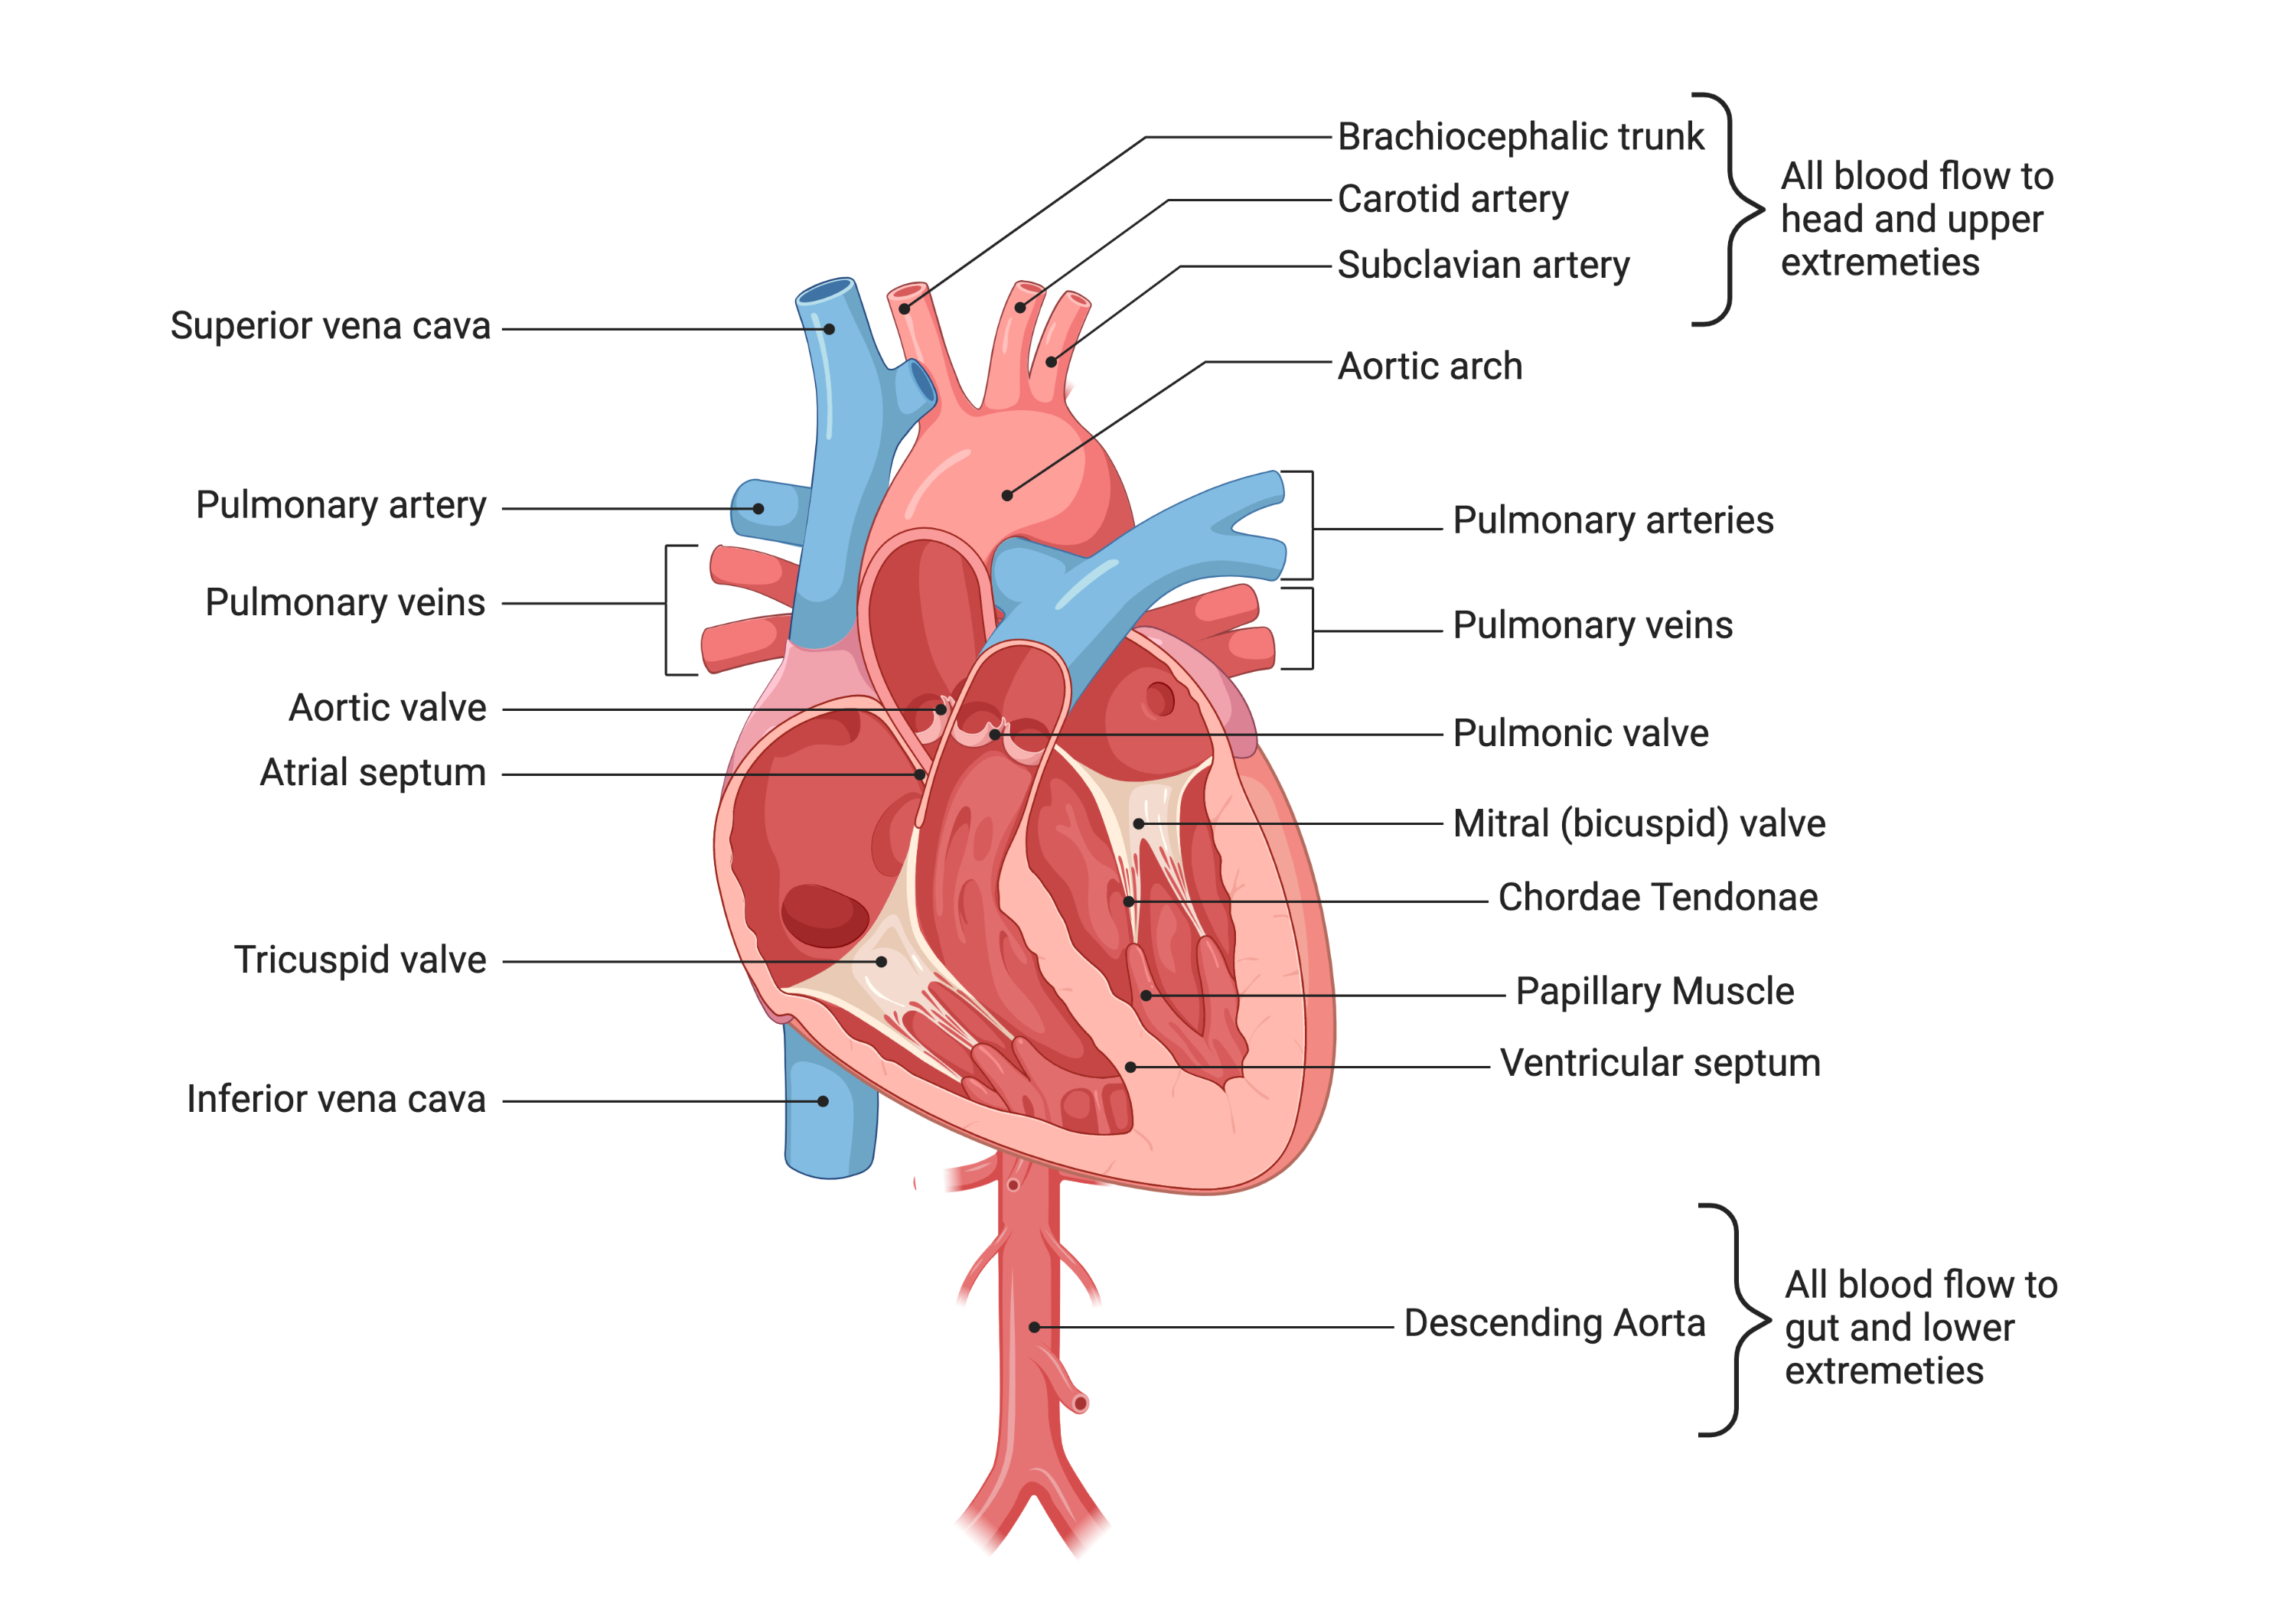
\includegraphics[width=1\linewidth]{./figure/Cardiac_Anatomy.png}
    \caption{Cardiac Anatomy \footnotesize{(Created with BioRender.com)}}
    \label{fig:Cardiac_Anatomy}
\end{figure}

Beyond being familiar with the structure in Figure \ref{fig:Cardiac_Anatomy} that are utilized throughout the chapter, there are several important structural takeaways.

\begin{itemize}
    \item Structurally there are four chambers, right and left atria (RA and LA); right and left ventricle (RV and LV) (the anatomical view).
    \item The four chambers form two primer-pumps for two circulations (right and left), RA and RV for the pulmonary circulation; and LA and LV for the systemic circulation (which includes all skeletal muscles and the heart itself) (the pump view).
    \item Cardiac muscle (myocardium) is thicker in the ventricles than the atria; and on the left side than the right side.
    \item The four chambers are divided into two excitation regions, RA and LA for atrial excitation; and RV and LV for ventricular excitation (the excitation view).
    \item The amount of tension and excitation is related to the thickness of the myocardium; which is based on how much pressure that chamber must generate for blood flow.
    \item Blood flow between the right and left primer-pumps is prevented by a septum (septal wall), also myocardium, that is thinner than the outer myocardial wall; and also thicker in the ventricles than the atria.
    \item Blood flow direction is guided by four one-way valves. Blood flow occurs due to pressure gradients - there is nothing inherently directional about pressure gradients other than high pressure to low pressure - therefore the valves are necessary to keep blood flowing from a chamber to the next chamber and now "backwards".
    \item All blood flow from the gut and lower extremity passes through the descending aorta; and comes to the heart through the inferior vena cava.
    \item All blood flow from the upper extremities and head passes through the great vessels (first three branches off of the aorta); and comes to the heart from the superior vena cava.
    \item For blood to flow through the circulation, venous pressure must be lower than arterial pressure
    \item Venous pressure (systemic in the RA; pulmonary in the LA) refers to the pressure that is the final end point for all venous blood flow returning to the heart which must, for blood flow to occur, have the lowest venous blood pressure of the respective circulations ($P_{RA} = 0$ when the RA is not generating tension). \item Ventricular systolic pressure refers to the pressure in the ventricles during active tensioning (contraction), for blood flow to occur it must have the highest arterial pressure of the respective circulations. The right sided ventricular systolic pressure is lower than the left sided ventricular systolic pressure, the respective circulations are considered low and high pressure.
    \item Because the ventricular systolic pressures must be the highest through the circulation, the tricuspid valve (between the RA and RV) and the bicuspid (mitral) valve (between the LA and LV) have additional support supplied by the papillary muscles and chordae tendonae (the support does not help them open, it prevents them from allowing backflow while closed).
    \item Because the LV has greater pressure than the RR, the mitral valve papillary muscle and chordae tendonae are more developed
    \item The aortic valve, which is not supported by papillary muscle, is under more pressure than the tricuspid valve because the aortic pressure is the second highest pressure in the circulation, however aortic peak pressure is short lived because of how rapidly blood flows out of the aorta.
\end{itemize}

\section{Blood Flow}

\subsection{Cardiac Output}

Blood flow (circulation) is measured and assessed based on the cardiac output ($\dot{Q}$) in liters (or mL) per minute. $\dot{Q}$ is directly proportional to the overall pressure gradient and inversely proportional to resistance to circulation:

\begin{equation}
    \dot{Q} = \frac{P_{a} - P_{RA}}{TPR}
    \label{Q}
\end{equation}

Where $P_{a}$ is pressure in the arteries (highest in the aorta); $P_{RA}$ is central venous pressure in the RA; and $TPR$ is the total peripheral resistance.

Since $P_{RA}$ normally approximates 0, the equation can be simplified to:

\begin{equation}
    \dot{Q} = \frac{P_{a}}{TPR}
    \label{Q_simplified}
\end{equation}

Another equation that is utilized to conceptualize $\dot{Q}$ is:

\begin{equation}
    \dot{Q} = HR \times SV
    \label{Q_HRSV}
\end{equation}

where HR is heart rate in beats per minute (bpm) and SV is stroke volume (the amount of blood pumped during systole) in mL. Which is simply the volume of blood ejected with each beat and the number of beats per minute to provide $\dot{Q}$ in mL/min.

\subsection{Blood Pressure}

Equation \ref{Q_simplified} can be manipulated to provide an equation for arterial pressure:

\begin{equation}
    P_{a} = \dot{Q} \times TPR
    \label{BP}
\end{equation}

Arterial pressure is blood pressure ($P_a$ = BP). Equation \ref{BP} shows that blood pressure is directly proportional to cardiac output and total peripheral resistance. 

Since the heart as a pump has two phases, a filling phase known as diastole, and a pumping phase known as systole it creates pulsatile flow. There is a rhythmic pulse in BP with a peak value referred to as systolic BP (SBP) and a low value referred to as diastolic BP (DBP). It is useful to consider SBP and DBP separately as well the mean arterial pressure (MAP):

\begin{equation}
    MAP = DBP + \frac{1}{3} \times (SBP - DBP)
    \label{MAP}
\end{equation}

Pulse pressure is the difference between SBP and DBP ($PP = SBP - DBP$, therefore Equation \ref{MAP}, can be simplified to:

\begin{equation}
    MAP = DBP + \frac{1}{3} \times PP
    \label{MAP_simplified}
\end{equation}

MAP is a weighted mean blood pressure. It is weighted by DBP more than SBP because the overall time period that the heart pump, and therefore the entire circulation, is in systole is much shorter than the overall time they are in diastole. With an increase in heart rate (HR) the time in systole becomes proportionally more time but the systolic time interval is relatively unchanged. The change in overall time in systole is based on there being less time in diastole. Despite this there is no modification to the equation for MAP during periods of higher HR.

\subsection{Poiseuille's Law}

Poiseuille's Law offers deeper insight into $\dot{Q}$ and Equation \ref{Q}.

\begin{equation}
    \dot{Q} = \frac{\Delta P \pi r^4}{\eta L}
    \label{Poiseuille}
\end{equation}

In Equation \ref{Poiseuille} $\dot{Q}$ is directly proportional to the pressure gradient as in Equation \ref{Q} as well as to the vessel cross sectional area squared. Area of a vessel is approximated by the area of a circle ($\pi r^2$), where $\pi$ is a constant and $r^2$ is the radius. Since flow is proportional to crosssectional area squared $(\pi r^2)^2$, it is proportional to radius to the 4th power ($\pi r^4$). $\dot{Q}$ is inversely proportional to the viscosity of the fluid ($\eta$) and the length of the vessel ($L$). 

Poiseuille's Law includes all the components of Equation \ref{Q}. $\Delta P$ is the pressure gradient between arteries (primarily aorta) and the right atria. Everything else in Equation \ref{Poiseuille} further elucidates components of TPR as resistance (R):

\begin{equation}
    R = \frac{\eta L}{\pi r^4}
    \label{resistance}
\end{equation}

The physiologically relevant variables of Equation \ref{Poiseuille} for blood flow are $\Delta P$, $r^4$ and $\eta$. $\pi$ is a constant and therefore does not contribute to our understanding of how blood flow changes. And for all intents and purposes $L$ is a constant. 

\subsection{Blood Flow Regulation}

Blood flow (circulation, $\dot{Q}$) regulation involves both quantity (how many liters / minute is being pumped) and distribution. Under normal circumstances all capillaries receive blood flow. However, the proportion of blood flow received in areas of the body is regulated. The regulation of $\dot{Q}$ quantity and distribution is coordinated because they must cooperate and because they include overlapping regulated variables. 

\paragraph{Vasovagal Syncope}
Vasovagal syncope is passing out, losing consciousness, due to a low blood pressure due to an emotional trigger. It is an example of a situation where there is not appropriate coordination between the regulation of $\dot{Q}$ and distribution. With vasovagal syncope many areas of the body are attempting to get more blood flow all at once (widespread vasodilation that reduces TPR) despite no increase in $\dot{Q}$. In this situation the BP drops enough that blood flow to the brain is reduced and there is a temporary loss of consciousness. The loss of consciousness usually results in a movement (falling) and a position (on the ground) that increases $\dot{Q}$ by increasing the amount of blood returning to the heart. Also, once unconscious the emotional trigger is no longer present and the vagal outflow that triggered a drop in TPR is removed, and reflexes that increase TPR in response to a drop in BP kick in to increase TPR. The combination of increased $\dot{Q}$ and TPR increase BP and restore brain blood flow (See Equation \ref{BP}.

\subsubsection{Blood Flow Regulation based on BP Regulation}

The regulation of blood flow is dependent on the regulation of blood pressure. From a regulation perspective Equation \ref{BP} is a starting point for understanding how blood flow regulation is achieved and how blood pressure is the primarily (but not exclusively\footnotemark\footnotetext{One notable exception to the regulation of blood flow by the monitoring of blood pressure is the kidneys, which regulate blood pressure by monitoring renal blood flow which is related to the glomerular filtration rate (GFR)}) monitored variable.

Expanding Equation \ref{BP} by adding the variables that determine $\dot{Q}$ and TPR we can derive a useful equation for thinking about blood flow regulation through blood pressure regulation.

\begin{equation}
    BP = (HR \times SV) \times \frac{\eta L}{\pi r^4}
\end{equation}

Since SV is the end diastolic volume (EDV) multiplied by the fraction of EDV ejected (EF) during systole:

\begin{equation}
    BP = (HR \times EDV \times EF) \times \frac{\eta L}{\pi r^4}
\end{equation}

Since $\eta$ (viscosity) is relatively stable, $L$ is very stable, and $\pi$ is a constant:

\begin{equation}
    BP = \frac{HR \times EDV \times EF}{r^4} 
    \label{BP_expanded}
\end{equation}

Maintaining BP requires maintaining blood flow ($\dot{Q} = HR \times EDV \time EF$) and includes regulating the radius of of blood vessels. Regulating the radius of blood vessels not only helps to create the gradient of high pressure at the heart and low pressure in the capillaries, but it is used to regulate the distribution of blood flow throughout the body.

The distribution of circulation is regulated by changing the radius of blood vessels. $r^4$ is inversely proportional to pressure and directly proportional to flow. Changes in vessel radius have a powerful influence over both so that increasing the radius decreases pressure and therefore increases flow to the 4th power. Decreasing radius increases pressure and therefore decreases flow to the 4th power. The flow down gradient of blood pressure from the heart to capillaries is largely based on the drop in pressure through the circulatory system due to a large increase in the overall radius (and volume) of arteries.

\paragraph{Vessel Compliance}

The above reasoning has left out - for the sake of simplicity - the concept of compliance. The regulation of vessel radius occurs through changes in vascular tone (smooth muscle in vessel walls, primarily arterioles to a lesser extent venuoles). Increased vascular tone decreases the radius and decreases its compliance. Therefore the increase in pressure goes beyond the reduction in cross-sectional area associated with the change in the radius. Decreased vascular tone increases the radius and increases its compliance. Therefore the decrease in pressure goes beyond the increase in cross-sectional area associated with the change in the radius. 

\paragraph{Per Minute to Per Cycle}

Equation \ref{BP_expanded} includes HR and therefore turns SV into $\dot{Q}$. The BP for a cardiac cycle ($BP_c$)can be considered by removing HR:

\begin{equation}
    BP_c = \frac{EDV \times EF}{r^4} 
    \label{BP_cycle}
\end{equation}

As a mean pressure, $BP_c$ can be considered based on the components of DBP and PP. In general, the DBP is influenced primarily by the TPR and thus the overall vessel radius. Therefore changes in DBP provides a general indication of changes in TPR. The additional pressure in the vessels during systole (SBP) is determined by adding PP to DBP (SBP = PP + DBP). Therefore PP changes in PP provides a general indication of changes in SV.

During progressively more intense exercise (a graded exercise test), despite linear increases in $\dot{Q}$ there is no change in DBP ($\pm$ 10 mmHg). This is due to large increases in the radius of blood vessels in working skeletal muscle and subsequent decreases in TPR. The large $\dot{Q}$ includes a larger SV (due to a larger EDV and equal (or slightly increased) EF). The larger SV produces a progressively larger PP, which produces increased SBP. When DBP, PP and SBP are being compared across multiple exercise intensities it is appropriate to reconsider the impact of Equation \ref{BP_expanded} since changes in BP across time that go beyond a several cycles (i.e. approaching minutes) more appropriately consider $\dot{Q}$ as opposed to SV.

Verification of the general phenomenon of DBP being indicative of TPR and PP (and therefore SBP) being indicative of SV and $\dot{Q}$ comes from studies on the differences in BP between upper extremity and lower extremity exercise. Lower PP (and therefore SBP), higher DBP, are achieved at any given submaximal HR during upper extremity as compared to lower extremity exercise despite a lower workload. Workload (in watts) provides a relatively stable estimate of the required oxygen and therefore $\dot{Q}$ \cite{dias_differences_2022}. Upper extremity exercise, despite a lower $\dot{Q}$ has a higher DBP because there are less, and smaller, arterioles dilating so there is a smaller increase in radius and therefore less reduction in TPR.

\subsection{Blood Flow Summary}

Throughout this chapter the cardiac and vascular factors that influence blood flow are covered at length. These factors all ultimately influence the variables in the equations of this section. They ultimately influence the pressure gradient generated by cardiac muscle tension and arteriole radius which influence volume, pressure, compliance and resistance to flow. Regulation BP is a major topic due to its centrality in the regulation of blood flow. Regulation of BP is also a major topic in Chapter \ref{chp:blood_content} on Blood Volume since not having enough blood makes it challenging to maintain BP and therefore blood flow.

\section{Cardiac Muscle}

The role of the heart as a pump is based on it's ability to regularly provide the pressure necessary for blood flow of blood through arterial vessels (both systemic arteries and pulmonary arteries). The function of the heart as a pump depends on several characteristics of cardiac muscle:

\begin{itemize}
    
    \item Automaticity: The ability to initiate its own excitation
    \item Rhythmicity: The ability to repeat the its own excitation cycle in synchrony with regularity
    \item Excitability: The ability to respond to excitation with activation
    \item Conductivity: The ability to transmit excitations from cell to cell within the heart
    \item Contractility: The ability to generate a full contractile (shortening) cycle with each excitation
 
\end{itemize}

\subsection{Tension}

It is reasonable to use the term contraction when describing activation and active tension for the cardiac muscle because contraction (shortening) is what occurs (there is no eccentric or isometric activation of cardiac muscle). A major difference between cardiac and skeletal muscle is that cardiac muscle does not have a tendon attachment. Cardiac muscle attaches to itself to create a chamber that has a volume. When cardiac muscle contracts, it makes the chamber smaller (less volume). In skeletal muscle the length of fibers translates into the length of the entire muscle and this relationship has a functional interpretation. In cardiac muscle the length of fibers directly translates into the volume of chambers. It is the volume of these chambers that has a functional interpretation. 

The heart has four chambers that function as four pumps (right and left atria; right and left ventricles). However from a muscular perspective there are two chambers, each separated into a right and a left side with a relatively thin muscular barrier between them. This is quite noticeable in conditions that result in abnormal timing of the right and left ventricle excitation. If the ventricles are not excited at the same time, off even by 50 milliseconds, the overall pump effectiveness of both ventricles is impaired.

\paragraph{Active Tension}

Active tension is generated in cardiac muscle with the same sliding filament model of skeletal muscle described in Chapter \ref{chp:tension}. Active tension generates tension that shortens cardiac muscle fibers and makes the cardiac chambers smaller (and less compliant). 

\paragraph{Passive Tension}

Passive tension is generated by titin and other connective tissue structures that resist lengthening of sarcomeres, which in turn resists enlarging the chamber. Passive tension also attempts to shorten cardiac muscle fibers when they are stretched (lengthened fibers when the chamber has a larger volume). Additional passive tension is developed by layers of connective tissue surrounding the heart including the epicardium (visceral layer of the serous pericardium), the parietal layer of the serous pericardium, and the fibrous pericardium (See Figure \ref{fig:Cardiac_Muscle}. The pericardial cavity is filled with pericardial fluid which reduces friction during the cardiac cycle of contraction - relaxation. All of these structures, including the amount of fluid in the pericardial fluid, impact the compliance of the heart chambers.

\begin{figure}[!h]
    \centering
    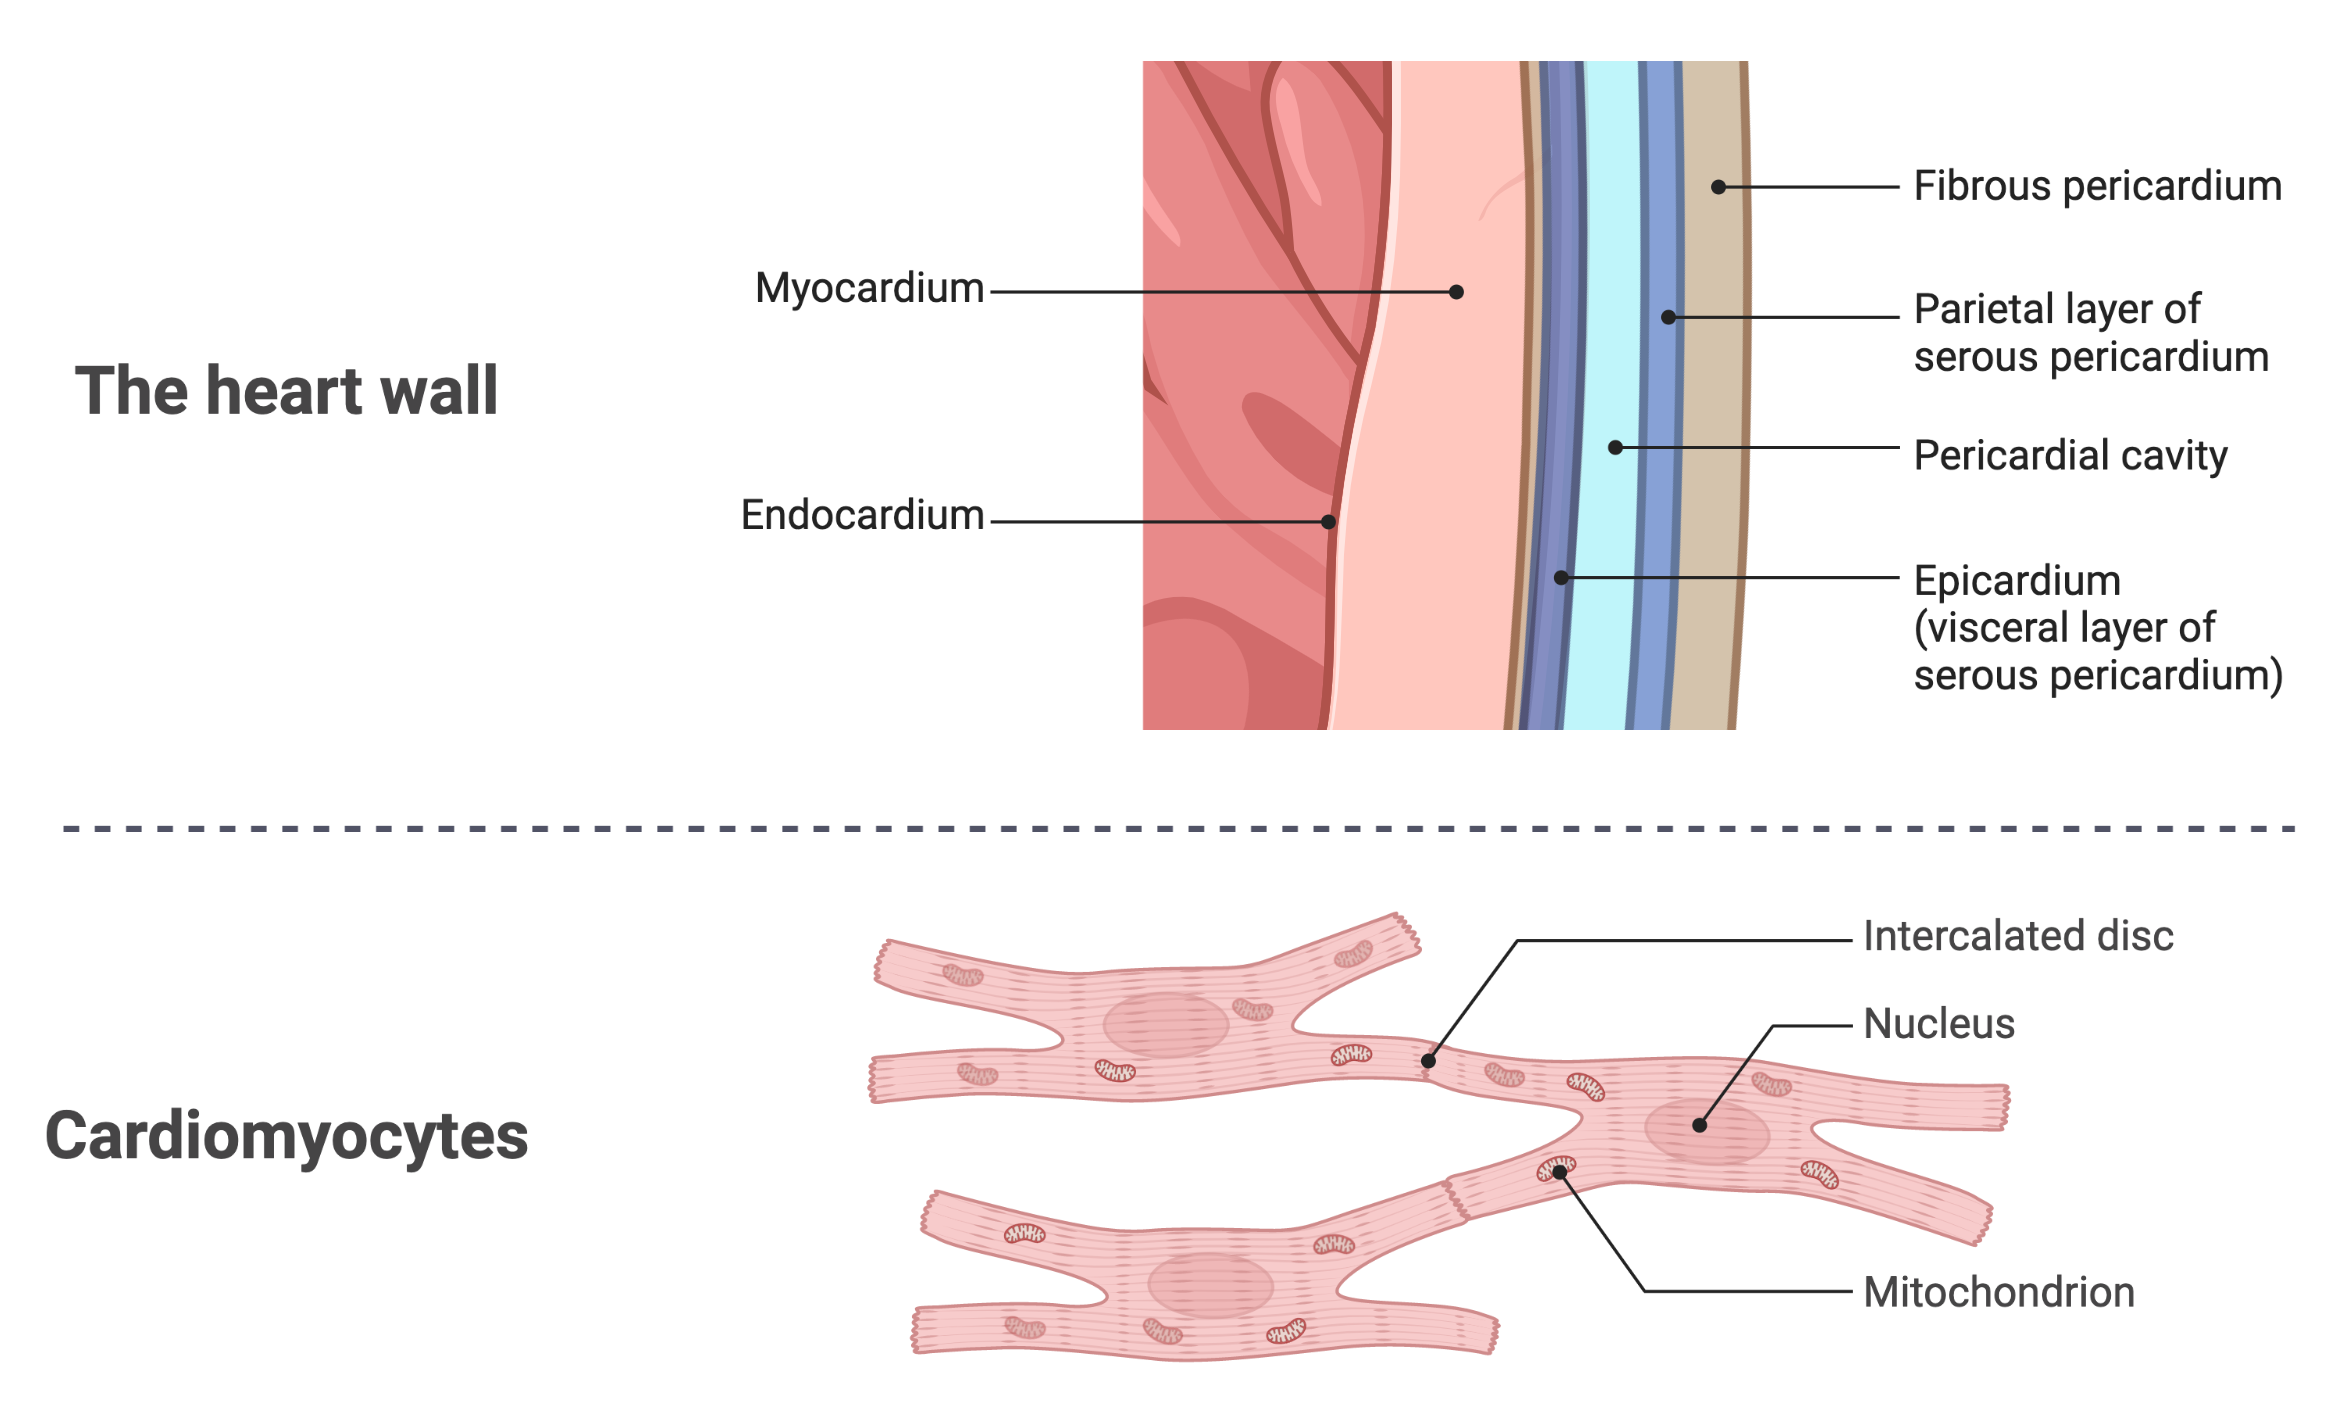
\includegraphics[width=1\linewidth]{./figure/Cardiac_Muscle.png}
    \caption{Cardiac Muscle \footnotesize{(Created with BioRender.com)}}
    \label{fig:Cardiac_Muscle}
\end{figure}

\paragraph{Volume-Tension Curve}

Cardiac muscle fibers \textit{in vitro} have a length-tension curve that is similar to skeletal muscle fibers. The primary difference is that the passive component is shifted to the left and is a steeper exponential curve. The active component displays a similar curve based on the overlap of actin and myosin. The passive component displays that cardiac muscle has a stiffer form of titin that contributes to tension with a smaller increase in length. 

Cardiac muscle \textit{in situ} has a volume-tension curve that is synonomous with the length-tension curve of whole skeletal muscle. The cardiac volume-tension curve is similar looking to its length-tension curve, the primary difference again being the passive component is shifted further to the left and is steeper. The volume-tension curve is influenced by the length-tension of the cardiac muscles and the passive structures surrounding the heart that resist changes in the chamber size directly. Passive tension starts to develop as the cardiac chamber fills. The functional implication is that even under normal resting conditions passive tension contributes to cardiac contraction. And with larger volumes of blood in the chambers the contribution of passive tension rises exponentially.

The passive component of the volume-tension curve is related to cardiac compliance. As described in Chapter \ref{chp:ecf_microcirculation} there is a relationship between volume, compliance and pressure. The cardiac muscles vary the volume of chambers while having a particular compliance (that varies with the passive and active tension) for the purpose of generating pressure. This is a fundamental difference between cardiac and skeletal muscle tension. Skeletal muscle tension changes length based directly on tension for the purposes of generating torque. Cardiac muscle tension changes length for the purpose of changing volume and compliance, for the purpose of changing pressure. It is the pressure generated in the cardiac chambers that result in blood flow.

Understanding cardiac function requires a familiarity with the equations relating compliance, volume and pressure introduced in Chapter \ref{chp:ecf_microcirculation}, repeated here:

\begin{equation}
    \Delta P_chamber = \frac{\Delta V_chamber}{C_chamber}
    \label{Cardiac_Pressure}
\end{equation}

In Equation \ref{Cardiac_Pressure} the dependency of pressure on volume and compliance is clear. Since blood flow (circulation) is a cyclic variation in pressure gradients through the cardiac pump (and vascular vessels), the entirety of cyclic blood flow through the heart can be considered from the perspective of cyclic changes to volume and compliance that develop pressure gradients to create flow through and out of the heart. Consideration of volume and compliance for the function of the heart a a pump correctly orients the discussion for both active and passive tension since they both contribute to cardiac pump function.

\subsubsection{Preload}

Preload is the term given for the pressure in a chamber when the cardiac muscle is filled (blood flow into the chamber is approaching 0) but is not yet activated. Preload is the passive tension in the chamber right before it develops active tension. Preload for cardiac muscle is analogous to stretch on skeletal muscle. The pressure of preload is related to the volume and the compliance. The compliance is at its highest when the myocardium is empty and not activated. As the chamber fills with blood, passive tension starts to develop which gradually reduces compliance while increasing the volume of blood, which combined increases pressure. Under normal circumstances this increase in pressure (higher blood volume and lower compliance) is not great enough to fully impede blood flow into the chamber. The passive tension developed during preload is subsequently utilized to assist active tension to develop the tension necessary to change the volume and compliance of the chamber for the purpose of increasing pressure to facilitate blood flow out of the chamber. The increased pressure, alone, simply directs blood flow out of the chamber from an area of high to low pressure. The direction of actual blood flow through the heart is dependent on properly functioning valves that limit flow "backwards" and allow blood flow "forwards" based on cardiac anatomy.

The preload is related most directly to what is referred to as end-diastolic pressure (EDP), which is related directly to end-diastolic volume (assuming the compliance is normal and relatively low during diastole). The volume that results in preload is from blood flow. Where the blood flow is coming from for preload depends on the chamber. The right artrium preload comes from the systemic veins; right ventricle preload comes from the right atrium through the tricuspid valve; left atrium preload comes from the pulmonary veins; left ventricle preload comes from the left atrium through the mitral valve. 

It is most common to discuss preload from the perspective of the left ventricle (LV). Therefore, unless otherwise noted EDV and EDP mean LVEDV and LVEDP (respectively). EDP is related to the \textbf{Frank-Starling mechanism} which states that the amount of venous return influences the performance of the left ventricle (assumes all the venous return moves through the right heart circulation (RA, RV, pulmonary arteries, pulmonary capillaries, pulmonary veins to the LA and finally the LV). The Frank-Starling mechanism is based on the relationship between EDP and total tension developed from active and passive tension.

\subsubsection{Afterload}
Afterload is the term given for the pressure that a chamber must overcome to cause blood flow out of the chamber. Afterload for cardiac muscle is analogous with resistance (or load) for skeletal muscle. It is the resistance that the cardiac chamber must exert its tension in order to reduce the volume of the chamber. The pressure of afterload depends on which chamber must overcome that pressure. For the RA it is the pressure exerted on the tricuspid valve by the RV; for the RV it is the pressure exerted on the pulmonic valve by the pulmonary arteries; for the LA it is the pressure exerted on the mitral valve by the LV; for the LV it is the pressure exerted on the aortic valve by the aorta (first of the systemic arteries). 

It is most common to discuss afterload from the perspective of the LV. Therefore, unless otherwise noted, afterload refers to aortic pressure and is best estimated as mean arterial pressure (MAP) (See Equation \ref{MAP_simplified}). MAP is related to specifically vascular compliance and resistance. As afterload, MAP affects aortic valve opening and is the most obvious load encountered by the ejecting ventricle. It should not be surprising that long term high blood pressure (hypertension) results in left ventricular hypertrophy (LVH) that tends to be associated with a reduced size and reduced compliance of the LV chamber. LVH is a common cause of diastolic (preserved ejection fraction) heart failure.

\paragraph{Ejection Fraction}

The amount of blood ejected from the LV during systole is called stroke volume (SV). It should be clear that SV is impacted by both preload and afterload. SV is simply the EDV minus the end systolic volume (ESV). 

The percentage of blood in the chamber (EDV) that is ejected during systole is the ejection fraction: 

\begin{equation}
    EF = \frac{ESV}{EDV}
    \label{LVEF}
\end{equation}

A useful equation to remember for SV is therefore:

\begin{equation}
    SV = EDV \times EF
    \label{SV}
\end{equation}

Equation \ref{SV} highlights how the two phases of the cardiac cycle (systole and diastole) contribute to stroke volume. Diastole contributes with a volume of blood (EDV). Systole contributes the tension to eject a fraction of that blood (LVEF). As discussed above, LVH can cause something called diastolic or preserved EF heart failure. That is because LVH reduces SV by reducing the size of the LV chamber. It reduces EDV, but does not reduce LVEF. There are also causes of HF that do reduce LVEF and they are called systolic or reduced EF heart failure. There are also situations - most often due to comorbidities (having more than one condition) - that cause HF with both diastolic (reduced EDV) and systolic (reduced LVEF) components. 

\paragraph{Rate Pressure Product}

The rate pressure product (RPP), also referred to as the double product, is described by the equation: $RPP = HR \times SBP$, where HR is heart rate and SBP is systolic blood pressure. It is an indication of cardiac muscle (myocardium) oxygen demand. This experimental observation has useful clinical application. It also demonstrates the fact that pressure generated by the myocardium includes active tension which requires oxygen.

In situations with increased afterload the myocardium must develop more pressure for blood flow. This greater pressure requires greater tension. This greater tension requires more ATP. More ATP requires more $O_2$. The more frequently the tension is generated (HR) the more ATP and subsequently $O_2$ is required. The experimental association between RPP and myocardial $O_2$ demand is a rather simple consequence of the underlying relationship between pressure (resistance), active tension and ATP.

If a patient undergoes maximal exercise testing and has myocardial ischemia, RPP can be calculated at the point when ischemia is occurring to establish the patient’s ischemic threshold. RPP at the ischemic threshold can then be used during exercise to provide a safe guideline of exercise intensity. This value is useful even if the patient is on a beta-adrenergic antagonist ($\Beta$-blocker). Even though the $\Beta$-blocker reduces the HR response by blocking the action of epinephrine and norepinephrine on the heart, it is this mechanism that reduces the risk of reaching ischemia. While on a $\Beta$-blocker, HR is not a good linear indication of overall aerobic workload (it loses its linear relationship with $\dot{V}O_2$), the RPP is a good discrete indicator of whether a patient is above or below their ischemic threshold. A patient that starts taking a $\Beta$-blocker (adrenergic antagonist) will have a harder time exceeding the ischemic threshold, which is the point of being on a $\Beta$-blocker for people with ischemic cardiac disease. 

% Revising stopped here on July 3rd

\subsection{Excitation}

To initiate a contraction cardiac muscle must undergo excitation. Excitation of cardiac muscle includes several similarities, but also differences, with skeletal muscle excitation. 

\subsubsection{Automaticity \& Rhythmicity}

Cardiac muscle is self excitatory (automaticity). Cardiac muscle self excitations are rhythmic, occurring at rest approximately every 40 seconds with very little variability when not influenced by the neuroendocine system (HR of approximately 90 bpm with low heart rate variability (HRV)). Or every 60 seconds with more variability when influenced by the neuroendocrine system at rest (HR of approximately 60 bpm with a HRV of approximately 50-100 ms when measured as a standard deviation with primarily parasympthatic influence).

Automaticity occurs (in normal conditions) in a cluster of myocardial cells in the right atrium known as the sino atrial (SA) node (pacemaker cells). Sino atrial node cells have a higher permeability to $Na^+$ than axonal or skeletal muscle membranes. Based on this higher permeability to $Na^+$ these cells do not have a sustained (stable) resting membrane potential (See Figure \ref{fig:Cardiac_SA_Node_AP}. As soon as their membrane is repolarized it begins a slow journey back to the threshold potential due to a slow influx of $Na^+$. How long it takes to reach the threshold (pacemaker potential) determines the heart rate. Under normal conditions the sino atrial node cells have the greatest pacemaker potential.

\begin{figure}[!h]
    \centering
    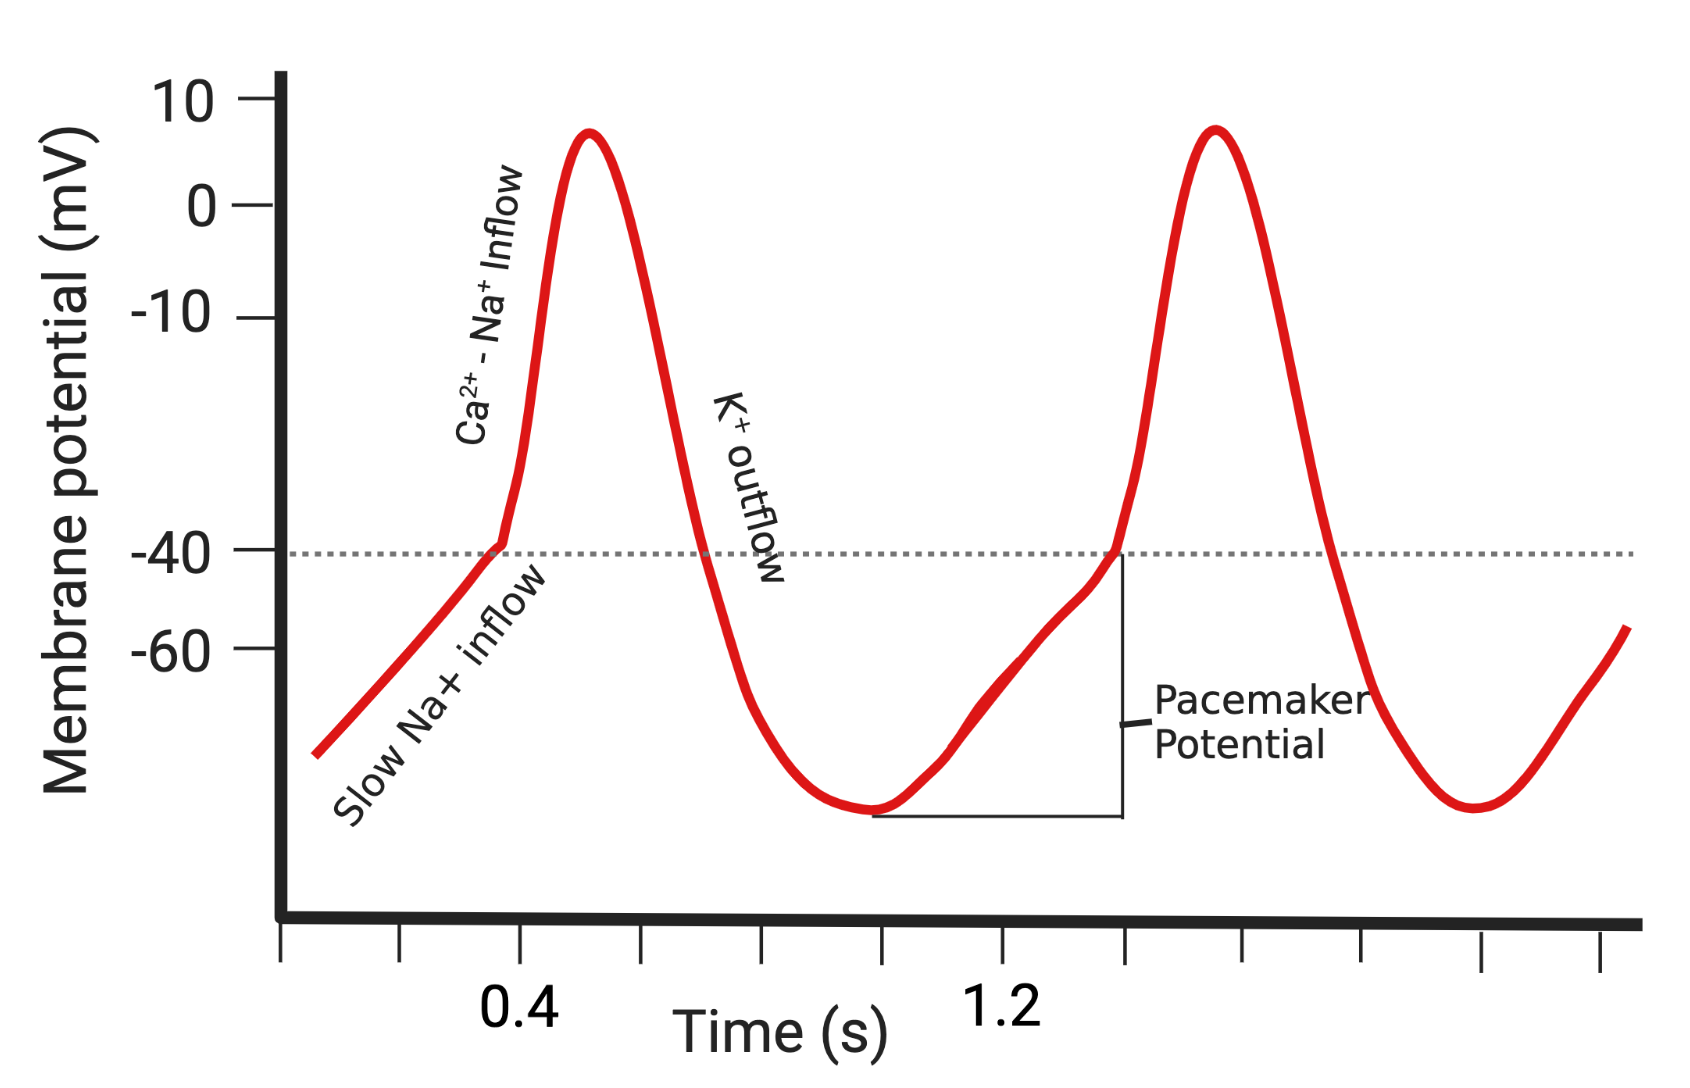
\includegraphics[width=0.5\linewidth]{./figure/Cardiac_SA_Node_AP.png}
    \caption{Cardiac Sino Atrial Node Excitation \footnotesize{(Created with BioRender.com)}}
    \label{fig:Cardiac_SA_Node_AP}
\end{figure}

\subsubsection{Conductivity} 

An excitation of the SA node results in full excitation of all the cardiac muscle cells, first in the atria, and then, after a delay, in the ventricles. There are three features of the myocardium that lead to this pattern of conductivity. 

\begin{figure}[!h]
    \centering
    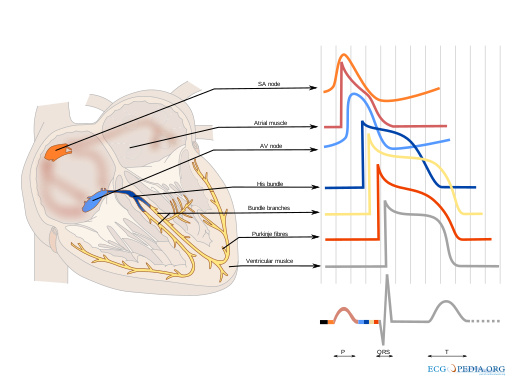
\includegraphics[width=1\linewidth]{./figure/Cardiac_Conduction.png}
    \caption{Cardiac Conduction \& Shapes of Excitation \footnotesize{(Created with BioRender.com)}}
    \label{fig:Cardiac_Conduction}
\end{figure}

First, there are specialized cardiac cells that form a conduction network (See Figure \ref{fig:Cardiac_Conduction}. The conduction network starts with the SA node sending a wave of excitation through the atria, facilitated by intra-nodal fibers (not shown in Figure \ref{fig:Cardiac_Conduction} that can rapidly carry an excitation from the SA node to the atrio-ventricular (AV) node. The excitation through the atria results in the P wave of the electrocardiograph (ECG). The excitation of the AV node and its distal conduction component, the bundle of His, is slower and delays the excitation of the ventricles (the PR interval on the ECG). Once through the AV node and bundle of His the excitation travels rapidly down the right and left bundle branches out to the purkinje fibers. The branching conduction network in the ventricles is critically important to rapid and synchronous excitation of the ventricles (the QRS complex in the ECG). Atrial repolarization is a minor event and is easily lost in the waves of the QRS. Ventricular repolarization is a more substantial event and results first in a return to baseline (ST segment on the ECG), and then the T wave on the ECG. It can also be noted in Figure \ref{fig:Cardiac_Conduction} that the AV node fibers have a pacemaker potential but it is smaller than the SA node pacemaker potential. The SA node is the pacemaker is the pacemaker under normal circumstances because it reaches the excitation threshold earlier than the AV node. However, if the SA node fails, the AV node reaches the excitation threshold and initiate ventricular excitation.

Second, there is a fibrous connective tissue boundary between the atria and the ventricles that does not transmit an excitation (does not have an excitable membrane). This helps ensure that ventricular excitation occurs only through excitation of the AV node (and no other way). The AV node ensures that the ventricular contraction occurs after a delay so that there is time for atrial contraction to push blood into the ventricles for the final stretch of the ventricles which facilitates more tension, thus more pressure for blood flow.

Third, each excitation travels from cardiac muscle fiber to the surrounding cardiac muscle fibers due to the presence of intercalated discs that have gap junctions between cardiac muscle fibers (See Figure \ref{fig:Cardiac_Gap_Junctions}. The presence of these gap junctions not only allows, but greatly expedites, the excitation of one fiber to the next. This is fundamentally different from skeletal muscle where each muscle fiber is insulated from nearby muscle fibers by the endomysium. In skeletal muscle such fiber to fiber excitation would be deleterious to controlled, coordinated movement. But in cardiac muscle this fiber to fiber wave of excitation facilitates the synchronized contraction of all atrial, and then ventricular fibers. Such "all together" contraction facilitates the change in atrial and ventricular chamber size which facilitates the change in pressure necessary for blood flow.

\begin{figure}[!h]
    \centering
    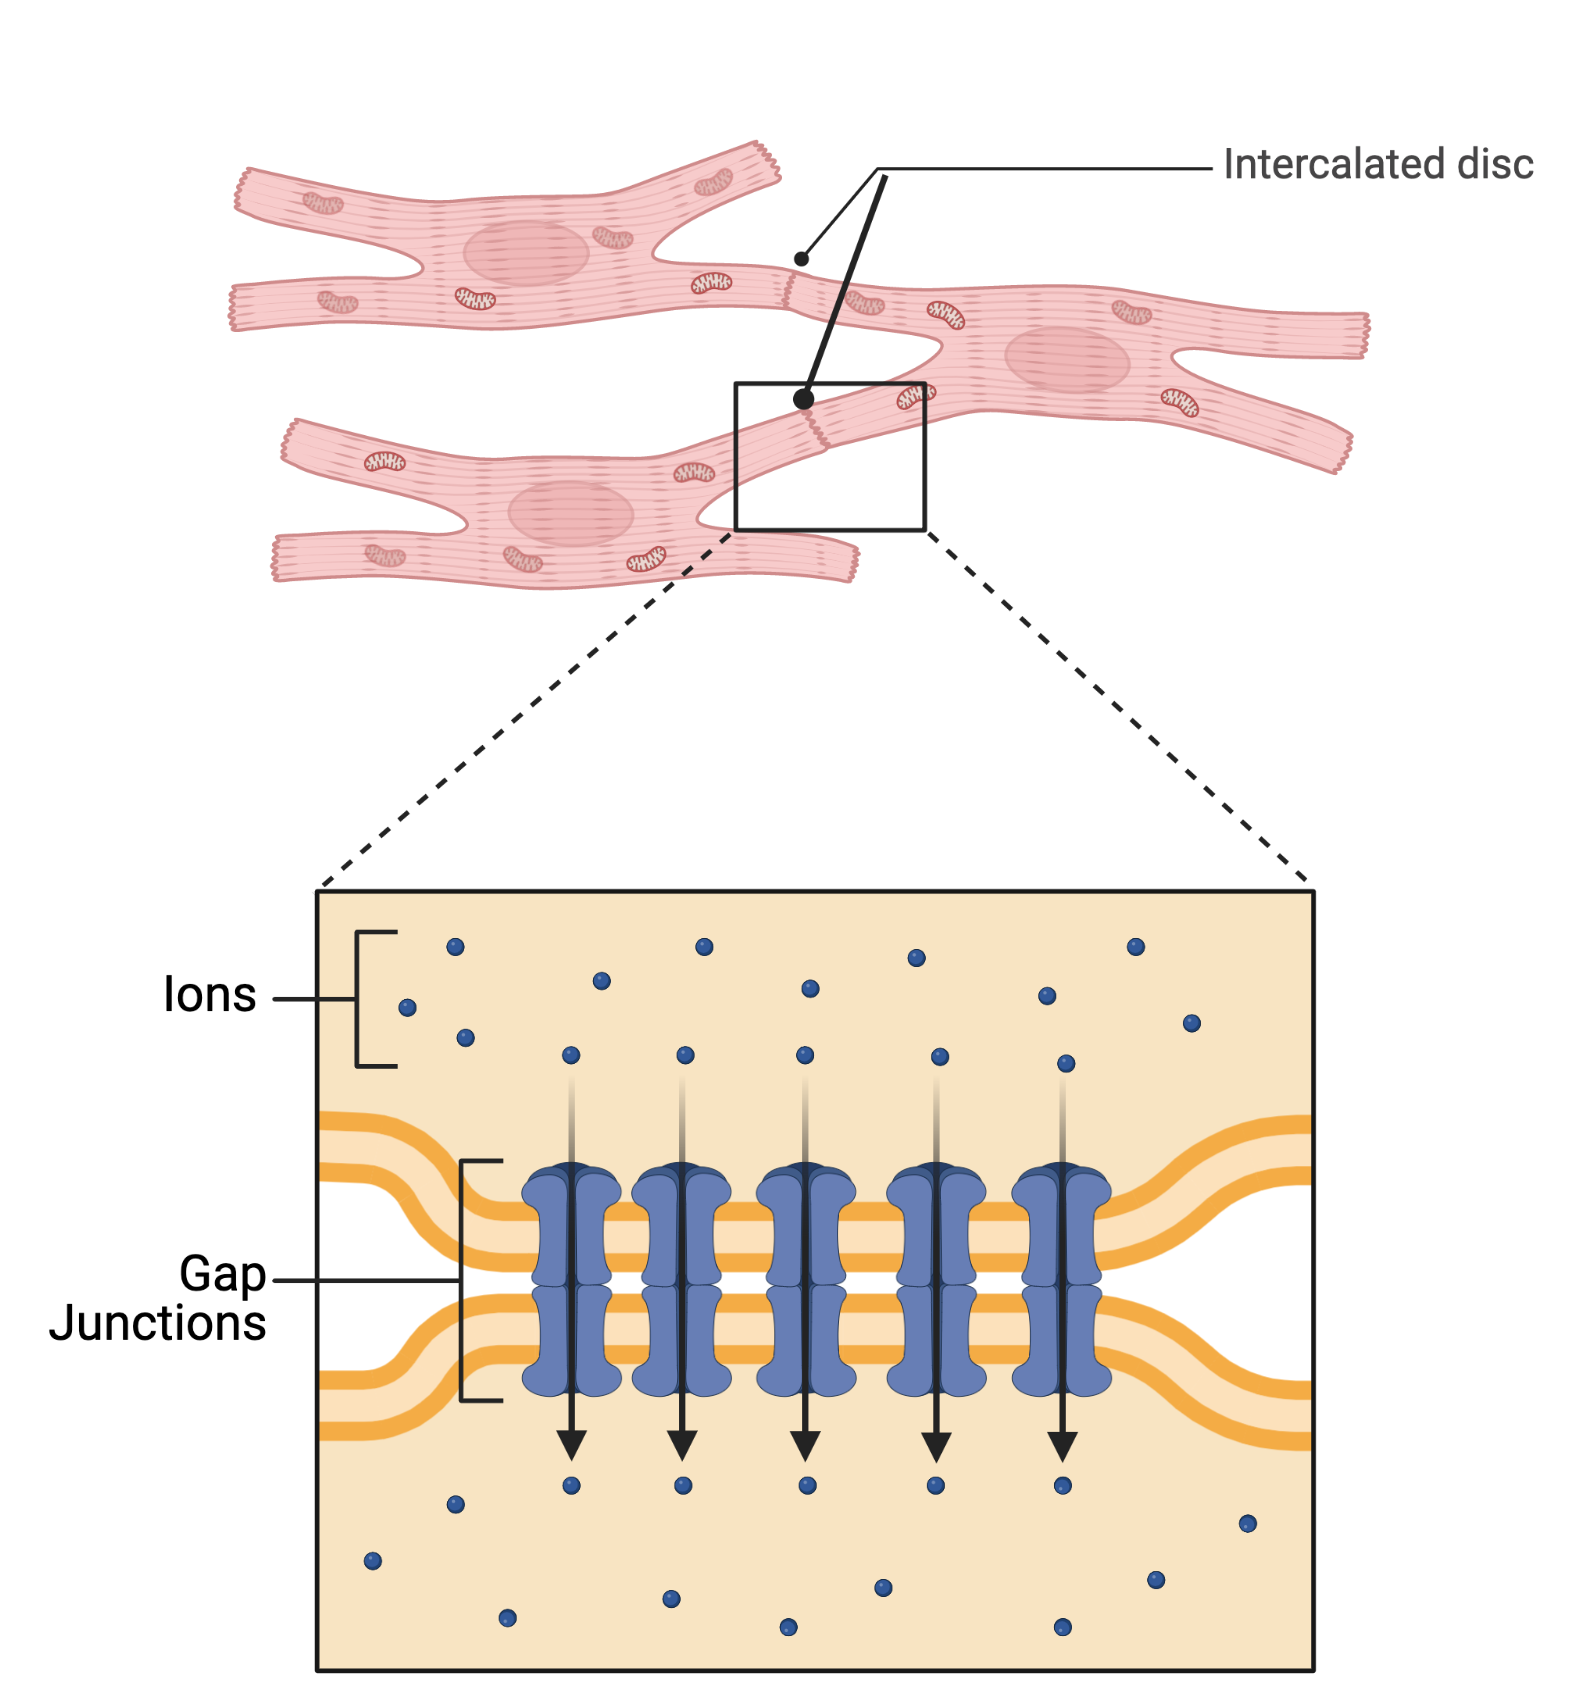
\includegraphics[width=0.5\linewidth]{./figure/Cardiac_Gap_Junctions.png}
    \caption{Intercalated Discs with Gap Junctions \footnotesize{(Created with BioRender.com)}}
    \label{fig:Cardiac_Gap_Junctions}
\end{figure}

\paragraph{Electrocardiogram (ECG)}

The wave of excitation through the cardiac conduction pathway and cardiac muscle fibers generates enough electrical potential to be measured by electrodes on the skin surface. There are several possible electrode placement arrangements, the most popular being referred to as a 12-lead ECG. The 12-lead ECG requires 10 electrodes. Four electrodes are on (or near) the limbs (six limb leads), and six electrodes are on the thorax and surround the heart (six precordial leads). Lead II arises from electrodes on the right arm and left leg and tracks the wave of excitation in the frontal plane from the sino atrial node (origin) through the left ventricle. The ECG wave from Lead II is the most commonly depicted ECG wave. Precordial ECG waveforms that are similar to Lead II include V4, V5 and V6.  Lead II, V4, V5 and V6 are commonly utilized for routine ECG monitoring for arrhythmias. 

A normal ECG is said to display sinus rhythm (sinus referring to the sino atrial node). Figure \ref{fig:ECG} displays the sinus rhythm waves of a normal ECG from the view of Lead II. Readers are encouraged to view videos of ECG in real time as a preferred approach to becoming familiar with rhythm analysis. A video of normal sinus rhythm is available at this \href{https://youtu.be/Q0JMfIVaDUE?list=PLNN6HI4OXQmyOMNWWrQCCQP559lvbcy4b}{link.}

\begin{figure}[!h]
    \centering
    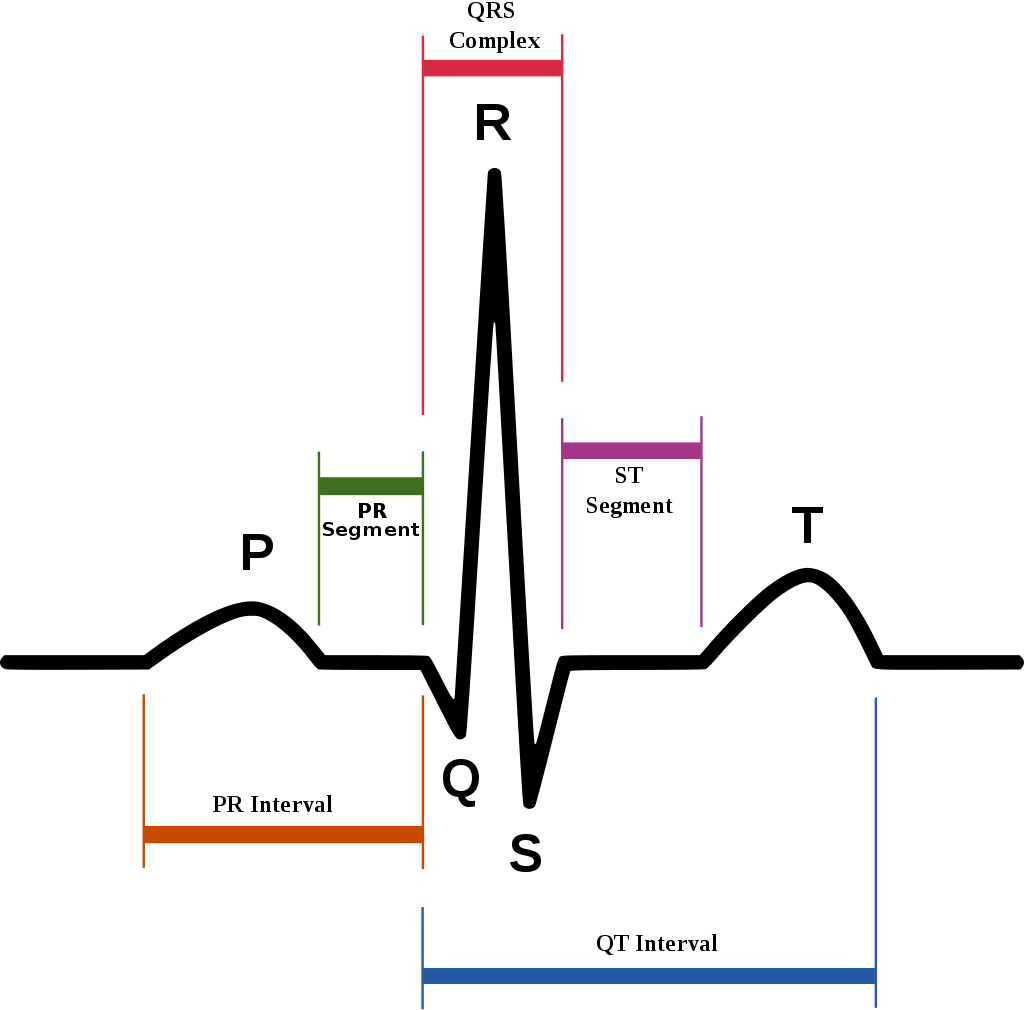
\includegraphics[width=0.5\linewidth]{./figure/ECG.png}
    \caption{ECG Waves (Lead II) \footnotesize{(From Wikipedia  \href{https://commons.wikimedia.org/wiki/File:SinusRhythmLabels.svg}{Sinus Rhythm Labels}, CC BY-SA 4.0)}}
    \label{fig:ECG}
\end{figure}

Table \ref{ECGWaves} refers to Figure \ref{fig:ECG} and provides further insight into the excitation event and clinical significance of each wave, segment and interval

\begin{table}[h!]
\centering
\begin{tabular}{||c c c ||} 
 \hline
 ECG & Excitation Event & Significance \\ [0.5ex] 
 \hline\hline
 P Wave & Atrial Depolarization & SA node, atria \\ 
 PR Segment & AV node delay & AV Node  \\
  PR Interval & SA \& AV node & SA \& AV node  \\
 QRS Complex & Ventricular Depolarization & Ventricles, RR Interval inversely proportional to HR  \\
 ST Segment & Ventricular Repolarization & Ischemia, Injury  \\
 QT Interval & Ventricular De + Repolarization & Long QT syndrome  \\ 
 T Wave & Ventricular Repolarization & Infarction \\ [1ex] 
 \hline
\end{tabular}
\caption{ECG Waves, Segments, Intervals and their excitation events and significance}
\label{ECGWaves}
\end{table}


\subsubsection{Contractility}

An excitation results in a full tetany of the myocardium that generate enough tension to generate enough pressure for blood flow. For a single excitation to result in full contraction of the atria and then the ventricles requires enough $Ca^{2+}$ to be released with one excitation for tetany (not just a twitch). There are two related features that allow for this to occur in cardiac muscle. 

First, the cardiac muscle excitation (action potential) is prolonged (See Figure \ref{fig:Cardiac_Ventricular_AP}). It is prolonged due to specialized voltage gated $Ca^{2+}$ channels that allow an inward movement of $Ca^{2+}$ following the initiation of the excitation by $Na^+$. The prolonged excitation occurs all the way down to the SR which continues to release $Ca^{2+}$. Second, it has also been proposed that the prolonged SR release of $Ca^{2+}$ into the cell also contributes to the prolonged excitation of the membrane itself (a positive feedback system). 

\begin{figure}[!h]
    \centering
    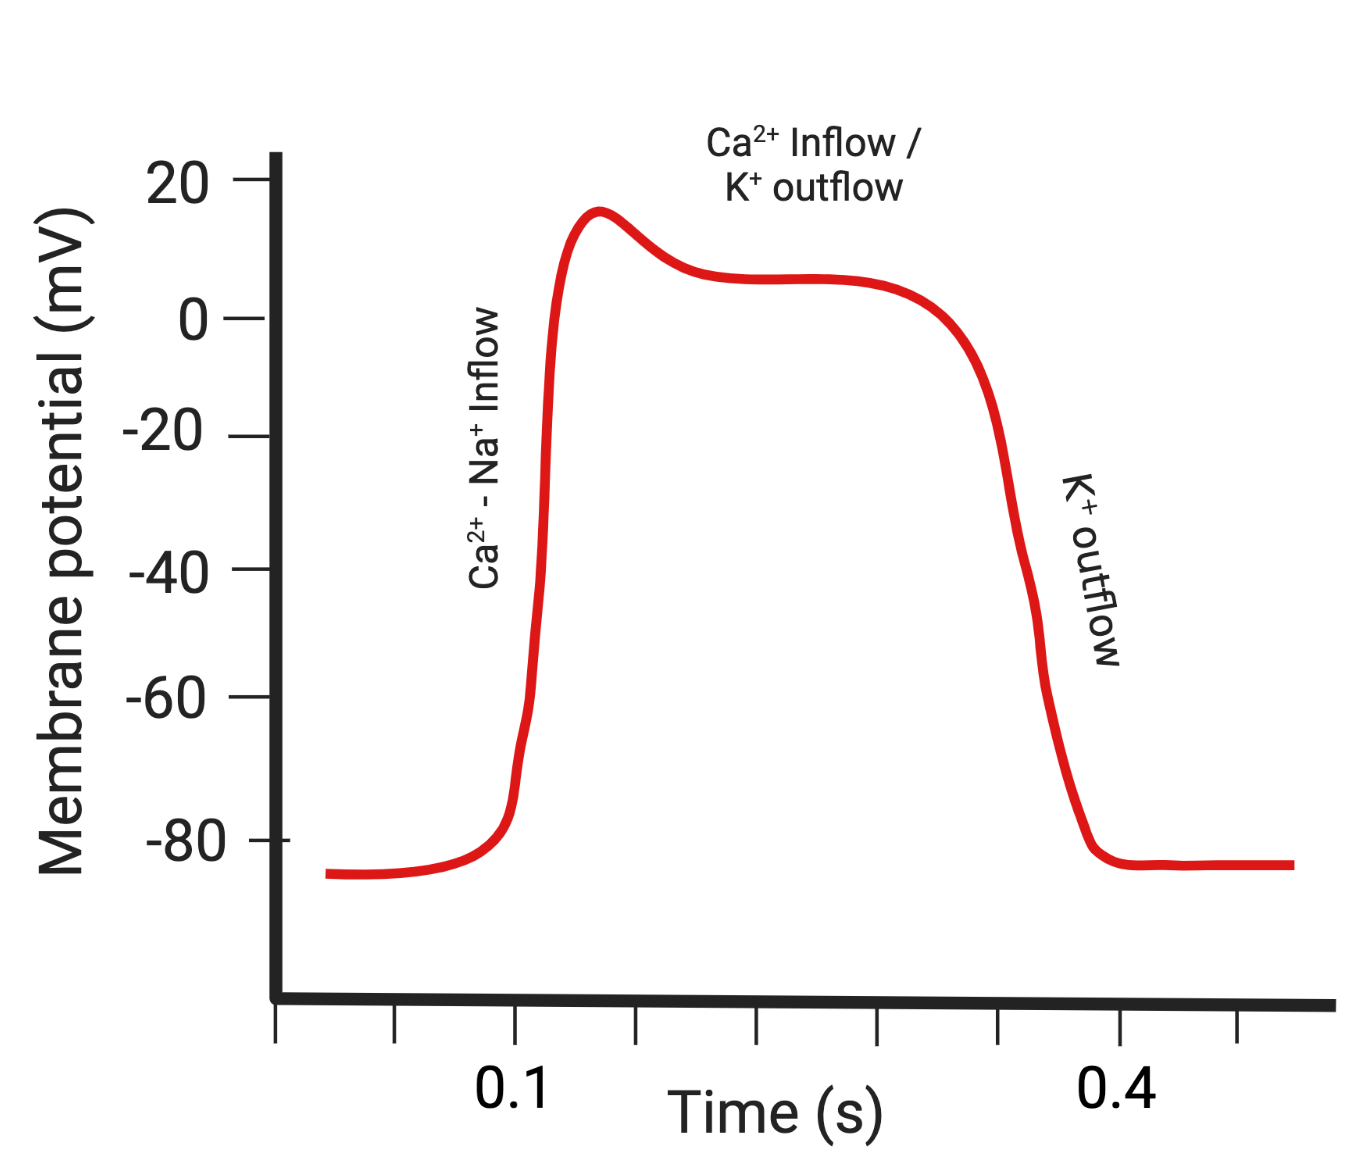
\includegraphics[width=0.5\linewidth]{./figure/Cardiac_Ventricular_AP.png}
    \caption{Ventricular Excitation \footnotesize{(Created with BioRender.com)}}
    \label{fig:Cardiac_Ventricular_AP}
\end{figure}

The primary take away message is that an excitation of a cardiac muscle fiber is prolonged due to inward movement of $Ca^{2+}$ across the sarcolemma, which leads to prolonged SR release of $Ca^{2+}$ for activation that also promotes prolonged excitation. Based on the importance of $Ca^{2+}$ in both prolonged excitation and activation of cardiac muscle fibers it should be of no surprise that medications that influence $Ca^{2+}$ make up two major classes of cardiac medications ($Ca^{2+}$-channel blockers which can either decrease the influx of, and/or the presence of $Ca^{2+}$; and digitalis, which increases the presence of $Ca^{2+}$ in the cardiac muscle fiber).


\subsection{Regulation}

There are two aspects to the regulation of cardiac output. The regulation of cardiac function (discussed here), and the regulation of distribution (discussed later).

A useful model of (equation for) cardiac output when considering regulation cardiac function is: 

\begin{equation}
    \dot{Q} = HR \times SV
    \label{Q_HRSV}
\end{equation}

For further consideration of cardiac function and cardiac output we can substitute SV with its components from Equation \ref{SV}:

\begin{equation}
    \dot{Q} = HR \times EDV \times LVEF
    \label{Q_HREDVEF}
\end{equation}

% Make a graphic on the regulation of cardiac function.

Based on Equation \ref{Q_HREDVEF} there are three possible ways for the cardiac output to be regulated by cardiac function.

\begin{enumerate}
    \item Regulate heart rate (HR)
    \item Regulation venous return (EDV)
    \item Regulate tension (contractility) (LVEF) 
\end{enumerate}

\subsubsection{Neuroendocrine Influence}

\paragraph{Neural Input}

The autonomic neuroendocrine system influences the heart via direct neural connections and through circulating hormones. It is important to keep in mind that the SA node is the pacemaker. The neuroendocrine input influences, but does not pace, the heart. The multitude of competing external influences to the pacing of HR is one of the reasons for the phenomenon known as HR variability (HRV). 

The parasympathetic (cholinergic) system has direct neural input through the cardiac branch of the vagal nerve (Cranial Nerve X). Vagal nerve activity generally decelerates cardiac function, thus decreasing HR, speed of the conduction wave of excitation and to a lesser extent contractility. The right vagus nerve stimulates primarily the SA node and affects rate, whereas the left vagus nerve stimulates primarily the AV node and affects AV conduction. Note that parasympathetic neural input does not influence EDV. 

Sympathetic (adrenergic) system neural input is through the thoracolumbar sympathetic system and increases HR and augments contractility, thus increasing cardiac function. The sympathetic nervous system also has connections to the peripheral vascular (arteries, arterioles, veins, venuoles). Therefore the sympathetic nervous system can change peripheral resistance, which changes vascular pressure and can alter venous return. Therefore, sympathetic influences can have a directly influences on EDV. 

Autonomic coordination: It should be noted that skeletal muscle activity has an influence over venous return. When the activity of these the sympathetic nervous system is coordinated with physical activity there is an increase in EDV due to increased skeletal muscle activity that compliments the other sympathetic influences. With the lack of sympathetic activity, and an increase in parasympathetic activity there is a decrease in EDV due to decreased skeletal muscle activity that compliments the other parasympathetic influences. 

\paragraph{Endocrine Input}
In response to physical activity or stress, the sympathetic nervous system also releases catecholamines (epinephrine and norepinephrine) from the adrenal cortex of the adrenal glands which increases HR, contractility, and total peripheral resistance for a net effect of increased cardiac function. Increased TPR has the effect of helping to facilitate venous return which then contributes to EDV.

\paragraph{Local Input}
Tissue pH, concentration of carbon dioxide ($CO_2$), concentration of oxygen ($O_2$), and metabolic products (e.g., lactic acid) can affect vascular tone. During exercise, increased levels of $CO_2$, decreased levels of $O_2$, decreased pH, and increased levels of lactic acid at the tissue level dilate local blood vessels and therefore increase $\dot{Q}$ distribution to that area.

\subsubsection{Cardiac Reflexes} % From ACH
Cardiac reflexes influence HR and contractility and can be divided into four general categories: baroreflex (pressure), Bainbridge reflex (stretch), chemoreflex (chemical reflex), ergoreflex (ergoreceptors). 

\paragraph{Baroreflex}

The baroreflex is activated through a group of mechanoreceptors located in the heart, great vessels, and intrathoracic and cervical blood vessels. These mechanoreceptors are most plentiful in the walls of the internal carotid arteries. Mechanoreceptors are sensory receptors that are sensitive to mechanical changes, such as pressure and stretch. Increased activity in the mechanoreceptors by high pressures increases vagal output and decreases sympathetic output. This chain of events results in vasodilation, decreased HR, and decreased contractility. The net effect is lower HR and SV, which reduce $\dot{Q}$ and therefore BP. Reduction in activity in the mechanoreceptors by low pressure results decreases vagal output and increases sympathetic output. This chain of events results in vasoconstriction, increased HR, and decreased contracility. The net effect is higher HR,  SV (as compared to lower sympathetic activity), which increase $\dot{Q}$ and therefore BP. The baroreflex is a quintesstential homeostatic negative feedback system - elevated BP promotes reduced BP, and reduced BP promotes elevated BP. It is the fast acting regulator of BP during body position changes that prevents syncope (loss of consciousness) during orthostatic challenges  (moving from supine to sit or standing).


\paragraph{Bainbridge Reflex}

Mechanoreceptors located in the right atrial myocardium respond to stretch. An increased volume in the right atrium results in an increase in pressure on the atrial wall. This reflex, known as the Bainbridge reflex, stimulates the vasomotor center of the medulla, which, in turn, increases sympathetic input and increases HR and contractility. Respiratory sinus arrhythmia, an increased HR during inspiration and decreased HR during expiration, may be facilitated by changes in venous return and SV caused by changes in thoracic pressure induced by the respiratory cycle. At the beginning of inspiration when thoracic pressure is decreased, venous return is greater; therefore a greater stretch is exerted on the atrial wall.

\paragraph{Chemoreflexes}
Chemoreceptors located on the carotid and aortic bodies have a primary effect on increasing rate and depth of ventilation in response to $CO_2$ levels, but they also have a cardiac effect. Changes in $CO_2$ during the respiratory cycle also may result in sinus arrhythmia.

\paragraph{Ergoreflexes}
Ergoreceptors and the ergoreflex regulates blood flow through activation of mechanosensitive afferents to inhibit the sustained vagal effects on the heart caused by an increase blood pressure triggering the baroreflex during physical activity that would otherwise work against the overall need for more circulation.

\subsection{Energetics}

Cardiac muscle is exceptionally well developed for aerobic metabolism, even more so than SO skeletal muscle fibers. Even during high intensity exercise cardiac muscle is capable of taking in lactate that is circulating in the blood and facilitating its transformation back into pyruvate and acetyl-CoA for entry into the citric acid cycle (TCA). Only when there is a lack of $O_2$ available for electron transport (ETC) do the aerobic energetic pathways not keep up with glycolosis in cardiac muscle cells. 

Cardiac muscle is so well developed for aerobic metabolism that even at rest the myocardium utilizes approximately 80\% of the $O_2$ delivered the blood. Skeletal muscle, at rest, only utilizes approximately 20\% of the $O_2$ that is delivered in the blood. This makes cardiac muscle critically dependent on increases in blood flow to provide the additional $O_2$ needed in response to increased myocardial oxygen demand (RPP).

To put this in context. If HR and SBP at rest are 60 beats per minute (bpm) and 110 mmHg then RPP is 6,600. If these values reach 180 bpm and 200 mmHg for an RPP of 36,000 there is a roughly a 5.5 fold increase in myocardial oxygen demand. To meet that demand a roughly 5 fold increase in myocardial blood flow (perfusion) must be achieved. This estimate is most accurate if these values are reached at rest (rare). If these values are achieved during exercise they are an over estimate of the actual myocardial oxygen demand. During exercise there is a significant increase in the skeletal muscle pumping action on venous circulation. Therefore there is a significant increase in venous return. Increased venous return increases preload. Increased preload increases the contribution of passive tension on cardiac contraction. The increased contribution of passive tension on cardiac contraction reduces the myocardial oxygen demand. 
Therefore, a HR of 180 and SBP of 200 at rest has a higher myocardial oxygen demand than a HR of 180 and SBP of 200 during exercise despite the same RPP because of the contribution of preload and passive tension to cardiac contractility.

% Left off here on Thursday morning June 30th

\section{Cardiac Cycle}

The events of the cardiac cycle are displayed in Figure \ref{fig:Cardiac_Wiggers}. 
\begin{figure}[!h]
    \centering
    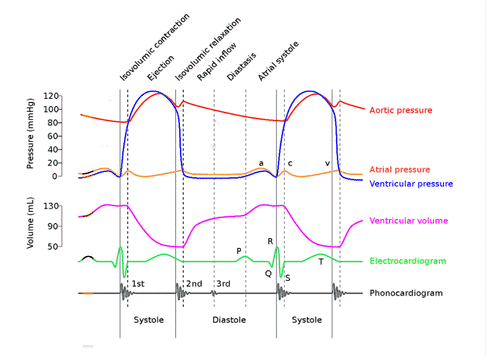
\includegraphics[width=1\linewidth]{./figure/Cardiac_Wiggers.png}
    \caption{Wiggers Diagram of the Cardiac Cycle \footnotesize{(From Wikipedia  \href{https://en.wikipedia.org/wiki/Wiggers_diagram}{Wiggers Diagram Entry}, CC BY-SA 4.0)}}
    \label{fig:Cardiac_Wiggers}
\end{figure}

Blood flow throughout the cardiac cycle depends on circulatory and cardiac pressure gradients. The right side of the heart is a low-pressure system with little vascular resistance in the pulmonary arteries, whereas the left side of the heart is a high-pressure system with high vascular resistance from the systemic circulation. The cardiac cycle is the period from the beginning of one contraction, starting with sinoatrial (SA) node depolarization, to the beginning of the next contraction. Systole is the period of contraction, and diastole is the period of relaxation. Systole and diastole can also be categorized into atrial and ventricular components.

\begin{itemize}
    \item Atrial diastole is the period of atrial filling. The flow of blood is directed by the higher pressure in the venous circulatory system.
    \item Atrial systole is the period of atrial emptying and contraction. Initial emptying of approximately 70\% of blood occurs as a result of the initial pressure gradient between the atria and the ventricles. Atrial contraction then follows, squeezing out the remaining 30\%.3 This is commonly referred to as the atrial kick.
    \item Ventricular diastole is the period of ventricular filling. It initially occurs with ease; then, as the ventricle is filled, atrial contraction is necessary to squeeze the remaining blood volume into the ventricle. The amount of stretch placed on the ventricular walls during diastole, referred to as left ventricular end diastolic pressure (LVEDP), influences the force of contraction during systole.
    \item Ventricular systole is the period of ventricular contraction. The initial contraction is isovolumic (i.e., it does not eject blood), which generates the pressure necessary to serve as the catalyst for rapid ejection of ventricular blood. The left ventricular ejection fraction (EF) represents the percent of end diastolic volume ejected during systole and is normally approximately 60\%.3
\end{itemize}

Understanding the cyclic events of Wiggers Diagram in Figure \ref{fig:Cardiac_Wiggers} requires an understanding of pressure changes due to volume and volume changes due to pressure. How these events are influenced by cardiac ac

\section{Circulation}

\subsection{Cardiac Output}
CO is the quantity of blood pumped by the heart in 1 minute. Regional demands for tissue perfusion (based on local metabolic needs) compete for systemic circulation, and total CO adjusts to meet these demands. Adjustment to CO occurs with changes in heart rate (HR—chronotropic) or stroke volume (SV—inotropic).4 Normal resting CO is approximately 4 to 8 liters per minute (L/min), with a resting HR of 70 beats per minute (bpm); resting SV is approximately 71mL/beat.3 The maximum value of CO represents the functional capacity of the circulatory system to meet the demands of physical activity.4
CO also can be described relative to body mass as the cardiac index (CI), the amount of blood pumped per minute per square meter of body mass. Normal CI is between 2.5 and 4.2L/min/m2. This wide normal range makes it possible for CO to decline by almost 40\% and still remain within the normal limits. Although several factors interrupt a direct correlation between CI and functional aerobic capacity,  CI below 2.5L/min/m2 represents a marked disturbance in cardiovascular performance and is always clinically relevant.5

\subsection{Cardiac Perfusion}

For a review of the major coronary arteries, refer to Fig. 3.1. Blood is pumped to the large superficial coronary arteries during ventricular systole. At this time, myocardial contraction limits the flow of blood to the myocardium; therefore myocardial tissue is perfused during diastole.

\subsection{Systemic Circulation}
For a review of the distribution of systemic circulation, refer to Fig. 3.4. Systemic circulation is affected by total peripheral resistance (TPR), which is the resistance to blood flow by the force created by the aorta and arterial system. Two factors that contribute to resistance are (1) vasomotor tone, in which vessels dilate and constrict; and (2) blood viscosity, in which greater pressure is required to propel thicker blood. TPR, also called systemic vascular resistance, and CO influence BP.3 This relationship is illustrated in the following equation:



\section{\textit{Practice Connections}} 

\subsection{ECG Rhythm Analysis}

ECG rhythm analysis allows identification of minor through major cardiac arrhythmias (conduction abnormalities) as well as deviations in wave forms that are associated with ischemia, injury or infarction of the myocardium (myocardial blood flow abnormalities). 

Rhythm analysis includes the observation of one ECG lead, usually in real time via a hard wired ECG monitor or a telemetry (wireless) ECG monitor. The first question when observing an ECG is whether it appears normal, that is with all of its waves and segments in order and spaced as expected. A general approach when observing the ECG in real time is to ask:

\begin{itemize}
    \item Is every P wave followed by a QRS?
    \item Is every QRS preceded by a P wave?
    \item Is every QRS followed by a T wave?
    \item Is every T wave preceded by a QRS?
    \item Is every T wave followed by a P wave?
    \item Is every P wave preceded by a T wave?
    \item Is the PR segment normal width?
    \item Is the QRS complex normal width?
    \item Does the ST segment quickly return to baseline?
    \item Are the QRS complexes reasonably and regularly spaced (RR Intervals)?
\end{itemize}


\subsubsection{Arrhythmias}

Examination for arrythmias can occur with any ECG lead (any one of the standard 12, or other less commonly used electrode and lead configurations). Every lead provides the same information about conduction. For example, if a P wave is missing or a PR interval is long in Lead II, it will be equally missing or as long in Lead aVL or V3 (or any of the other leads). 

\paragraph{Tachyarrythmias (Ectopy)}

Tachyarrythmias refer to arrhythmias associated with more excitation than usual during cardiac conduction. Such aberrant excitation usually results in a higher heart rate. Tachycardia is a HR higher than 100 bpm and is not technically an arrhythmia - though if its occurs without provocation (physical, mental or emotional stress) then it may be indicative cardiac or autonomic dysfunction. When tachycardia is unprovoked it is often referred to as supra-ventricular tachycardia (SVT) or atrial tachycardia. The most common type of SVT is paroxysmal SVT (PSVT). Paroxysmal simply means it comes and goes without any currently understood provocation (cause).
There are a group of tachyarrythmias caused by ectopic action potentials that cause ectopic excitations and beats. Ectopic simply means these excitations are not originating in the SA node and following the normal excitation conduction pathway. Ectopy originates from an ectopic focus (myocardial cells causing an action potential) or if more than one focus, as ectopic foci. An ectopic focus (or foci) can occur due to myocardial cell irritation (producing an excitation when it should not, i.e. caffeine or other stimulants), or due to myocardial cell depression (delay or block in conduction (ischemia, injury or scar tissue) that produces a recurrent loop of self perpetuating excitation within the myocardium). 

Table \ref{Tachyarrhythmia} organizes six different tachyarrhythmias based on where they occur (atria or ventricles) and the regularity of the ectopic focus (or foci) excitations.

\begin{table}[h!]
\centering
\begin{tabular}{||c c c ||} 
 \hline
   & Atria & Ventricle \\ [0.5ex] 
 \hline\hline
 Occasional Ectopic Focus & Premature Atrial Contr. (PACs) & Premature Ventricular Contr. (PVCs)\footnotemark\footnotetext{Also referred to generally as ventricular ectopy or ventricular premature beats (VPBs)} \\ 
 Occasional Ectopic Foci & PACs & Multifocal PVCs \\
 Non Stop Ectopic Focus & Atrial Flutter (AFlutter)& Ventricular Tachycardia (VTach)  \\
 Non Stop Ectopic Foci & Atrial Fibrillation (AFib) & Ventricular Fibrillation (VFib)  \\ [1ex] 
 \hline
\end{tabular}
\caption{Types of Ectopic Tachyarrhythmia}
\label{ECGWaves}
\end{table}

As with all conduction abnormalities the severity of a tachyarrhythmia is based on the impact it has on hemodynamics (cardiac output and blood pressure). In general that impact is greater proceeding down the rows; and is always greater in the ventricular column than the atrial column. For example, PACs have little, if any, impact on hemodynamics; whereas VFib does not produce any blood flow at all so there is no cardiac output and no blood pressure (and therefore no pulse). 

Since the tachyarrhytmias exist on a spectrum, it is required that a physical therapist can identify which tachyarrhytmia is present should one arise (or be part of a patient's chronic condition). For example, it is not appropriate to stop activity due to AFib in a patient with chronic AFib. Nor is it required to stop activity due to PACs or PVCs in all situations. 

A YouTube playlist of tachyarrhythmias is available at this \href{https://www.youtube.com/playlist?list=PLNN6HI4OXQmwFdE8LVIGC_l5WG2ViWAy3}{link.}

\paragraph{Bradyarrythmias \& Blocks}

Bradycardia refers to any HR below 50 bpm. However, like tachycardia, bradycardia does not always indicate there is a conduction problem. Whether bradycardia is a problem comes down to whether it is creating problems with hemodynamics. Generally, if there is an abnormality causing bradycardia it will provoke problematic changes in hemodynamics, for example, sick sinus syndrome or third degree AV block. A normal cause of bradycardia that does not provoke problematic changes in hemodynamics is being well conditioning from exercise training.

Bradyarrhythmias can be caused by AV blocks, though not all instances of AV blocks create bradycardia. It is just common to classify blocks as a bradyarrhythmia. There are three degrees of AV Block, and four types (there are two types of second degree AV block.

\begin{itemize}
    \item First Degree AV Block: Prolonged PR Interval
    \item Second Degree AV Block - Mobitz 1 (Wenkebach) - progressive prolongation of the PR interval until finally there is a P wave without a QRS indicating the conduction was blocked which is then followed by a normal PR interval that begins progressive prolongation (this pattern repeats)
    \item Second Degree AV Block - Mobitz 2 - normal PR interval with an occasional P wave with no QRS
    \item Third Degree AV Block - complete AV block (also referred to as complete heart block) P waves and aberrant looking QRS complexes are completely dissociated (though may occasionally align so identification requires watching the ECG for several cycles)
\end{itemize}

A YouTube playlist of bradyarrhythmias and AV blocks is available at this \href{https://www.youtube.com/playlist?list=PLNN6HI4OXQmyt5Ql2um3MthEtLkdJnywd}{link.}

The severity of AV blocks is related to the impact they have hemodynamics. As can be expected, the severity increases from First Degree to Third Degree. Mobitz 2 is considered more severe to Mobitz 1, not due to hemodynamic differences, but because it is more likely to deteriorate into Third Degree AV block.

\subsection{Myocardial Blood Flow Abnormalities}

Abnormalities in myocardial blood flow (perfusion) such as ischemia lead to hypoxic conditions in the myocardial cells. If the ischemia persists cell death will occur. Prior to cell death an early indication of ischemia includes changes to the ST segment of the ECG. In a very general way, ST changes are indicative of ischemia and/or injury. This more general fact is sometimes made more specific, with ST depression taken as a sign of myocardial ischemia and ST elevation taken as a sign of myocardial injury. Myocardium that is injured may be reversibly injured (will recover) or irreversibly injured (will die, infarction). 

A YouTube playlist of ST segment changes is available at this \href{https://www.youtube.com/playlist?list=PLNN6HI4OXQmyHL-CDiLqrBSkv6E1Vk0cS}{link.}

One of the problems with the more specific claims of ST changes is that it assumes the ECG lead being observed is a lead that has the best view of the myocardium that has ischemia. Unlike the the arrhythmias which are seen equally well in all ECG leads, a blood flow abnormality resulting in ischemia is local to the region of the myocardium with the blood flow abnormality (rarely the entire myocardium). For example, aVR tends to have a reversed polarity to Lead II (what goes up in Lead II goes down in aVR, what goes down in Lead II goes up in aVR). If ischemia is in an area that Lead II shows depression, it may appear as elevation in aVR. During the diagnostic process (a cardiac stress test) a 12 lead ECG is utilized and additional testing strategies are utilized to confirm that what was observed was in fact ischemia. A cardiologist can get a good idea of where the ischemia is occurring from the 12-lead ECG, which is then confirmed with imaging (nuclear scans or catheterization). When it is known which location (and therefore lead) best pin points the area with a propensity for ischemia then that lead (or a couple of leads) can be utilized for rhythm monitoring. In such situations it is mostly true that ischemia appears as ST depression, and injury appears as ST elevation.

Since the physical therapist using rhythm analysis is primarily interested in identifying abnormalities that warrant the cessation of activity and alerting members of the medical team of such abnormalities (not in making a diagnosis), simply identifying ST changes is sufficient. Both ischemia and injury are sufficient reason to stop activity and alert members of the medical team. In fact, the risk associated with myocardial ischemia and injury is sufficient to warrant extra caution and stopping activity if ST changes are suspected while observing the ECG rhythm. In other words, if the ST segment appears above or below the baseline its safer to assume it is than to assume it isn't. Cease activity and continue monitoring. As with any such signs, noting other signs and symptoms is warranted (shortness of breath, diaphoresis, chest pain, blood pressure, respiratory rate).

\subsection{Cardiovascular Vital Signs}

\subsubsection{Palpation of Pulses} 
Palpation of pulses is an important component of a physical examination and can be used to evaluate and identify the following:

\begin{itemize}
\item Circulation quality
\item Pulse rate and rhythm
\end{itemize}

\paragraph{Circulation Quality}

Pulse are pressure waves through the circulation that are related to both blood pressure and local circulation. Weak pulses can indicate either low blood pressure (overall) or poor blood flow that particular region of the body. For example, a weak pulse in the right radial artery but not the left radial artery most likely indicates a local blood flow problem in the left UE but not the right. Whereas a weak pulse in all extremities is most likely a low blood pressure overall. A strong, or bounding, pulse can indicate a high blood pressure overall, or a high blood pressure in a particular area. Bounding pulses can also indicate vascular abnormalities such as aneurysms (for example a bounding abdominal pulse is a sign of a descending aortic aneurysm).

\paragraph{Heart Rate \& Rhythm}

Pulses are correlated with heart rate (cardiac cycle) and rhythm. When palpating a pulse to obtain HR, counting the pulse rate for 15 seconds and multiplying by 4 is sufficient with normal rates and rhythms. If rates are faster than 100 bpm or slower than 60 bpm, palpate the pulse for 60 seconds. If the rhythm is irregularly irregular (e.g., during AFib) or regularly irregular (e.g., PACs or PVCs), perform auscultation of heart sounds to identify the apical HR for a full minute. In these cases, palpation of pulse cannot substitute for ECG analysis to monitor the patient’s rhythm, but it may alert the therapist to the onset of these abnormalities.

Use caution in palpating pulses because manual pressure on the carotid sinus may cause baroreflex drops in heart rate (HR), blood pressure (BP), or both. In all pulse palpation situations the examiner should start with light pressure and gradually increase pressure until a pulse is felt, and to not exert more pressure than required to feel the pulse.

Some people can feel a pulse in their thumb, therefore it is generally advised to not use the thumb to palpate a pulse.

HR is the primary means of determining the exercise intensity level for patients who are not taking beta-blockers or who have rate-responsive pacemakers. HR combined with blood pressure (RPP) is the most appropriate approach to determine exercise intensity in any patient with a known ischemic threshold (even if they are on beta-blockers).

\begin{itemize}
\item A linear relationship exists between HR and work.
\item In general, a 20- to 30-beat increase from the resting value during activity is a safe intensity level in which a patient can exercise.
\item If a patient has undergone an exercise stress test during the hospital stay, a percentage (e.g., 60\%–80\%) of the maximum HR achieved during the test can be calculated to determine the exercise intensity.
\item An example of a disproportionate HR response to low-level activity (bed or seated exercises or ambulation in room) is an HR of more than 120bpm or less than 50bpm.
\item HRR, which provides an indication of reduced parasympathetic activity and an indicator of all-cause mortality, can be used to document improvement of tolerance to functional demands.83 HRR is the absolute difference between peak HR achieved with exercise minus the HR at 60 seconds after the completion of exercise (HRR 60sec).  An abnormal HRR at 1 minute, after a treadmill test, is reported to be a decrease of 12bpm or less with a cool-down period and less than 18bpm without a cool-down period.
\item When prescribing activity intensity for a patient taking beta-blockers, consider that HR should not exceed 20 beats above the resting HR. If RPP for the patient's ischemic threshold is known, then the RPP should not be allowed to increase to the ischemic threshold.
\item If prescribing an activity intensity, with use of HR, for patients with an AICD, remember that the exercise target HR should be 20 to 30 beats below the threshold rate on the defibrillator.82
\item HR should not be used to prescribe exercise status post heart transplantation secondary to denervation of the heart during transplantation.
\item Baseline HR and recent changes in medications always should be considered before beginning an exercise session.
\end{itemize}

\subsubsection{Blood Pressure}

Blood pressure is critical to blood flow and one of the variables utilized to help regulate cardiac output (baro reflex). Low blood pressure (and low pulse pressure) is problematic because it compromises blood flow and may indicate hemodynamic compromise due to cardiac (reduced cardiac output), vascular (reduced peripheral resistance) or blood volume problems. High blood pressure can create immediate health care emergencies by placing blood vessels under too much pressure; or cardiac emergencies by causing ischemia (high RPP and myocardial $O_2$ demand), or heart failure (increased afterload). Long term increased high blood pressure (hypertension) leads to long term changes in the heart (left ventricular hypertrophy, fibrosis of the atria and ventricles that makes the heart more susceptible to arrhythmias, or valve dysfunction). Hypertension is a silent killer since many individuals have no idea they have it - which is one of the reasons for the APTA Academy of Cardiovascular and Pulmonary Physical Therapy's "Vitals are Vital" campaign to encourage all physical therapists in all settings to make sure they routinely examine vitals signs in all clients.

Measurement of BP with a sphygmomanometer (cuff) and auscultation is an indirect, noninvasive measurement of the force exerted against the arterial walls during ventricular systole (systolic blood pressure [SBP]) and during ventricular diastole (diastolic blood pressure [DBP]). BP is affected by total peripheral resistance (blood volume, radius and elasticity of arterial walls) and cardiac output ($\dot{Q}$). Table \ref{table:BP} lists normal BP ranges. 

\begin{table}[h!]
\centering
\begin{tabular}{||c c c ||} 
 \hline
 Ranges & Systolic (mmHg) & Diastolic (mmHg) \\ [0.5ex] 
 \hline\hline
Age 8 years & 85-114  & 52-85  \\ 
Age 12 years & 95-135  & 58-88   \\
Adult & < 120   & < 80   \\
Elevated (Adult) & 120-129   & < 80  \\
Stage 1 Hypertension & 130-139  & 80-89   \\
State 2 Hypertension & $\geq$ 140 &  $\geq$ 90 \\ [1ex] 
 \hline
\end{tabular}
\caption{Blood Pressure Ranges}
\label{BP}
\end{table}

Occasionally, BP measurements can be performed only on certain limbs secondary to the presence of such conditions as a percutaneously inserted central catheter, arteriovenous fistula for hemodialysis, blood clots, scarring from brachial artery cutdowns, or lymphedema (e.g., status post mastectomy). 

BP of the upper extremity should be measured in the following manner: \cite{collins_cardiac_2019}

\begin{enumerate}
\item Check for posted signs, if any, at the bedside that indicate which arm should be used in taking BP. BP variations of 5 to 10 mmHg between the right and left upper extremity are considered normal. Patients with arterial compression or obstruction may have differences of more than 10 to 15 mmHg.
\item Use a properly fitting cuff. The inflatable bladder should have a width of approximately 40\% and length of approximately 80\% of the upper arm circumference.
\item Position the cuff 2.5 cm above the antecubital crease.
\item Rest the relaxed arm at the level of the heart.
\item To determine how high to inflate the cuff, palpate the radial pulse, inflate until no longer palpable, and note the cuff inflation pressure. Deflate the cuff. This is an estimate of the systolic pressure. But this method cannot be utilized to obtain a diastolic pressure.
\item Place the bell of the stethoscope gently over the brachial artery.
\item Reinflate the cuff to 30 to 40 mmHg greater than the value in step 5. Then slowly deflate the cuff. Cuff deflation should occur at approximately 2 to 3 mmHg per second.15
\item Listen for the onset of tapping sounds, which represents blood flow returning to the brachial artery. This is the SBP.
\item As the pressure approaches diastolic pressure, the sounds will become muffled and in 5 to 10mmHg will be completely absent. These sounds are referred to as Korotkoff sounds (See Table \ref{Korotkoff}).
\end{enumerate}

\begin{table}[h!]
\centering
\begin{tabular}{||c c c ||} 
 \hline
 Phase & Korotkoff Sound & Indicates \\ [0.5ex] 
 \hline\hline
1  & First sound, faint tapping  & Systolic pressure (blood flow through compressed artery)  \\ 
2  & Blowing or swishing sound  & Blood is increasing   \\
3 & Distinct tapping 0   & Blood flow is increasing   \\
4 & Muffled  & Diastolic pressure in certain situations$^a$\\
5 & Disappearance  & Diastolic pressure in adults   \\ [1ex] 
 \hline
\end{tabular}
\caption{Blood Pressure Ranges ($^a$ \footnotesize{Phase 4 represents DBP in children, and adults that are exercising, pregnant or with hyperthyroid conditions})(Modified from \cite{bickley_bates_2012})}a
\label{Korotkoff}
\end{table}

\paragraph{Systolic Blood Pressure / Palp}

In situations when it is difficult to auscultate or to obtain a distinct diastolic blood pressure reading (DBP), the palpation method may be utilized and blood pressure is noted as systolic blood pressure (SBP)/Palp. This is the same procedure utilized in Step 5 to determine how high to pump the cuff for a full measurement of blood pressure without having to over inflate the cuff.


\subsection{Physical Therapy Considerations}
\begin{itemize}
\item Recording pre exertion, para exertion, and post exertion BP is important for identification of BP responses to activity. During recovery from exercise, blood vessels dilate to allow for greater blood flow to muscles. In cardiac-compromised or very deconditioned individuals, total $\dot{Q}$ may be unable to support this increased flow to the muscles and may lead to decreased output to vital areas, such as the brain.
\item If you are unable to obtain BP on the arm, the thigh is an appropriate alternative, with auscultation at the popliteal artery.
\item Falsely high readings occur if the cuff is too small or applied loosely or if the brachial artery is lower than the heart level.
\item Evaluation of BP and HR in different postures can be used to monitor orthostatic hypotension with repeat measurements on the same arm 1 to 5 minutes after position changes.
\item The same extremity should be used when serial BP recordings will be compared for an evaluation of hemodynamic response.
\item A BP record is kept on the patient’s vital sign flow sheet. This is a good place to check for BP trends throughout the day and, depending on your hospital’s policy, to document BP changes during the therapy session.
\item An auscultatory gap is the disappearance of sounds between phase 1 and phase 2 and is common in patients with high BP, venous distention, and severe aortic stenosis. Its presence can create falsely low SBPs if the cuff is not inflated enough (prevented by palpating for the disappearance of the pulse before measurement), or falsely high DBPs if the therapist stops measurement during the gap (prevented by listening for the phase 3 to phase 5 transitions).
\item In general there is a lower SBP, higher DBP, and lower workload at any given submaximal HR during arm exercise compared with leg exercise \cite{dias_differences_2022}
\item A clearly disproportionate response to exercise includes SBP decrease of 10 mmHg below the resting value, a hypertensive systolic response of greater than 200 mmHg, or a hypertensive diastolic response of greater than 110 mmHg. A normotensive systolic blood response should increase 5 to 12 mmHg per increase in metabolic equivalents (METs).\footnotemark\footnotetext{One MET is approximately 3.5 ml/kg/min of oxygen consumption.}
\item If the patient is on a pacemaker that does not have rate modulation, BP response can be used to gauge intensity. 
\end{itemize}

\section{Summary}

\subsection{Next Step}

\printbibliography[heading=subbibintoc]